\documentclass[twoside]{book}

% Packages required by doxygen
\usepackage{fixltx2e}
\usepackage{calc}
\usepackage{doxygen}
\usepackage[export]{adjustbox} % also loads graphicx
\usepackage{graphicx}
\usepackage[utf8]{inputenc}
\usepackage{makeidx}
\usepackage{multicol}
\usepackage{multirow}
\PassOptionsToPackage{warn}{textcomp}
\usepackage{textcomp}
\usepackage[nointegrals]{wasysym}
\usepackage[table]{xcolor}

% Font selection
\usepackage[T1]{fontenc}
\usepackage[scaled=.90]{helvet}
\usepackage{courier}
\usepackage{amssymb}
\usepackage{sectsty}
\renewcommand{\familydefault}{\sfdefault}
\allsectionsfont{%
  \fontseries{bc}\selectfont%
  \color{darkgray}%
}
\renewcommand{\DoxyLabelFont}{%
  \fontseries{bc}\selectfont%
  \color{darkgray}%
}
\newcommand{\+}{\discretionary{\mbox{\scriptsize$\hookleftarrow$}}{}{}}

% Page & text layout
\usepackage{geometry}
\geometry{%
  a4paper,%
  top=2.5cm,%
  bottom=2.5cm,%
  left=2.5cm,%
  right=2.5cm%
}
\tolerance=750
\hfuzz=15pt
\hbadness=750
\setlength{\emergencystretch}{15pt}
\setlength{\parindent}{0cm}
\setlength{\parskip}{3ex plus 2ex minus 2ex}
\makeatletter
\renewcommand{\paragraph}{%
  \@startsection{paragraph}{4}{0ex}{-1.0ex}{1.0ex}{%
    \normalfont\normalsize\bfseries\SS@parafont%
  }%
}
\renewcommand{\subparagraph}{%
  \@startsection{subparagraph}{5}{0ex}{-1.0ex}{1.0ex}{%
    \normalfont\normalsize\bfseries\SS@subparafont%
  }%
}
\makeatother

% Headers & footers
\usepackage{fancyhdr}
\pagestyle{fancyplain}
\fancyhead[LE]{\fancyplain{}{\bfseries\thepage}}
\fancyhead[CE]{\fancyplain{}{}}
\fancyhead[RE]{\fancyplain{}{\bfseries\leftmark}}
\fancyhead[LO]{\fancyplain{}{\bfseries\rightmark}}
\fancyhead[CO]{\fancyplain{}{}}
\fancyhead[RO]{\fancyplain{}{\bfseries\thepage}}
\fancyfoot[LE]{\fancyplain{}{}}
\fancyfoot[CE]{\fancyplain{}{}}
\fancyfoot[RE]{\fancyplain{}{\bfseries\scriptsize Generated by Doxygen }}
\fancyfoot[LO]{\fancyplain{}{\bfseries\scriptsize Generated by Doxygen }}
\fancyfoot[CO]{\fancyplain{}{}}
\fancyfoot[RO]{\fancyplain{}{}}
\renewcommand{\footrulewidth}{0.4pt}
\renewcommand{\chaptermark}[1]{%
  \markboth{#1}{}%
}
\renewcommand{\sectionmark}[1]{%
  \markright{\thesection\ #1}%
}

% Indices & bibliography
\usepackage{natbib}
\usepackage[titles]{tocloft}
\setcounter{tocdepth}{3}
\setcounter{secnumdepth}{5}
\makeindex

% Hyperlinks (required, but should be loaded last)
\usepackage{ifpdf}
\ifpdf
  \usepackage[pdftex,pagebackref=true]{hyperref}
\else
  \usepackage[ps2pdf,pagebackref=true]{hyperref}
\fi
\hypersetup{%
  colorlinks=true,%
  linkcolor=blue,%
  citecolor=blue,%
  unicode%
}

% Custom commands
\newcommand{\clearemptydoublepage}{%
  \newpage{\pagestyle{empty}\cleardoublepage}%
}

\usepackage{caption}
\captionsetup{labelsep=space,justification=centering,font={bf},singlelinecheck=off,skip=4pt,position=top}

%===== C O N T E N T S =====

\begin{document}

% Titlepage & ToC
\hypersetup{pageanchor=false,
             bookmarksnumbered=true,
             pdfencoding=unicode
            }
\pagenumbering{roman}
\begin{titlepage}
\vspace*{7cm}
\begin{center}%
{\Large Tiny\+Comp\+: a toy compiler for C\+S5500 }\\
\vspace*{1cm}
{\large Generated by Doxygen 1.8.11}\\
\end{center}
\end{titlepage}
\clearemptydoublepage
\tableofcontents
\clearemptydoublepage
\pagenumbering{arabic}
\hypersetup{pageanchor=true}

%--- Begin generated contents ---
\chapter{Hierarchical Index}
\section{Class Hierarchy}
This inheritance list is sorted roughly, but not completely, alphabetically\+:\begin{DoxyCompactList}
\item \contentsline{section}{Address}{\pageref{class_address}}{}
\begin{DoxyCompactList}
\item \contentsline{section}{Const\+Address}{\pageref{class_const_address}}{}
\item \contentsline{section}{Instr\+Address}{\pageref{class_instr_address}}{}
\item \contentsline{section}{Temp\+Address}{\pageref{class_temp_address}}{}
\item \contentsline{section}{Var\+Address}{\pageref{class_var_address}}{}
\end{DoxyCompactList}
\item \contentsline{section}{Attribute}{\pageref{class_attribute}}{}
\begin{DoxyCompactList}
\item \contentsline{section}{Bool\+Attr}{\pageref{class_bool_attr}}{}
\item \contentsline{section}{Expr\+Attr}{\pageref{class_expr_attr}}{}
\item \contentsline{section}{Stmt\+Attr}{\pageref{class_stmt_attr}}{}
\end{DoxyCompactList}
\item \contentsline{section}{fraction}{\pageref{structfraction}}{}
\item \contentsline{section}{Memory}{\pageref{class_memory}}{}
\item \contentsline{section}{Sym\+Tbl}{\pageref{class_sym_tbl}}{}
\begin{DoxyCompactList}
\item \contentsline{section}{Simple\+Array\+Sym\+Tbl}{\pageref{class_simple_array_sym_tbl}}{}
\end{DoxyCompactList}
\item \contentsline{section}{Tac\+Instr}{\pageref{class_tac_instr}}{}
\item \contentsline{section}{Target\+Code}{\pageref{class_target_code}}{}
\end{DoxyCompactList}

\chapter{Data Structure Index}
\section{Data Structures}
Here are the data structures with brief descriptions\+:\begin{DoxyCompactList}
\item\contentsline{section}{\hyperlink{class_address}{Address} }{\pageref{class_address}}{}
\item\contentsline{section}{\hyperlink{class_attribute}{Attribute} }{\pageref{class_attribute}}{}
\item\contentsline{section}{\hyperlink{class_bool_attr}{Bool\+Attr} }{\pageref{class_bool_attr}}{}
\item\contentsline{section}{\hyperlink{class_const_address}{Const\+Address} }{\pageref{class_const_address}}{}
\item\contentsline{section}{\hyperlink{class_expr_attr}{Expr\+Attr} }{\pageref{class_expr_attr}}{}
\item\contentsline{section}{\hyperlink{structfraction}{fraction} }{\pageref{structfraction}}{}
\item\contentsline{section}{\hyperlink{class_instr_address}{Instr\+Address} }{\pageref{class_instr_address}}{}
\item\contentsline{section}{\hyperlink{class_memory}{Memory} }{\pageref{class_memory}}{}
\item\contentsline{section}{\hyperlink{class_simple_array_sym_tbl}{Simple\+Array\+Sym\+Tbl} }{\pageref{class_simple_array_sym_tbl}}{}
\item\contentsline{section}{\hyperlink{class_stmt_attr}{Stmt\+Attr} }{\pageref{class_stmt_attr}}{}
\item\contentsline{section}{\hyperlink{class_sym_tbl}{Sym\+Tbl} }{\pageref{class_sym_tbl}}{}
\item\contentsline{section}{\hyperlink{class_tac_instr}{Tac\+Instr} }{\pageref{class_tac_instr}}{}
\item\contentsline{section}{\hyperlink{class_target_code}{Target\+Code} }{\pageref{class_target_code}}{}
\item\contentsline{section}{\hyperlink{class_temp_address}{Temp\+Address} }{\pageref{class_temp_address}}{}
\item\contentsline{section}{\hyperlink{class_var_address}{Var\+Address} }{\pageref{class_var_address}}{}
\end{DoxyCompactList}

\chapter{File Index}
\section{File List}
Here is a list of all documented files with brief descriptions\+:\begin{DoxyCompactList}
\item\contentsline{section}{\hyperlink{tinycomp_8h}{tinycomp.\+h} \\*This header file contains the definitions that must be shared between flex, bison, and the support code }{\pageref{tinycomp_8h}}{}
\item\contentsline{section}{\hyperlink{tinycomp_8hpp}{tinycomp.\+hpp} \\*This header file contains the support code for the translator of tinycomp }{\pageref{tinycomp_8hpp}}{}
\end{DoxyCompactList}

\chapter{Data Structure Documentation}
\hypertarget{class_address}{}\section{Address Class Reference}
\label{class_address}\index{Address@{Address}}


{\ttfamily \#include $<$tinycomp.\+hpp$>$}

Inheritance diagram for Address\+:\begin{figure}[H]
\begin{center}
\leavevmode
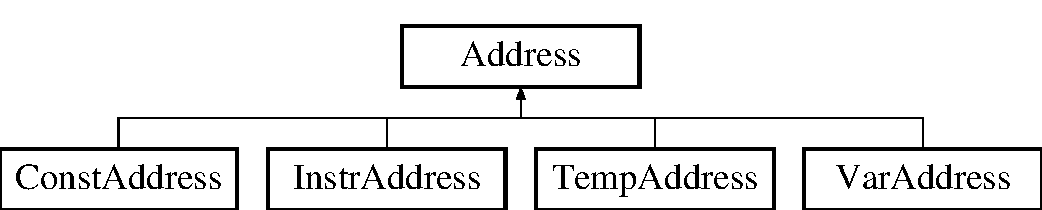
\includegraphics[height=2.000000cm]{class_address}
\end{center}
\end{figure}
\subsection*{Protected Member Functions}
\begin{DoxyCompactItemize}
\item 
virtual const char $\ast$ \hyperlink{class_address_ac58183c3d3dc7c3e98a17825dd086de1}{to\+String} () const =0
\end{DoxyCompactItemize}
\subsection*{Friends}
\begin{DoxyCompactItemize}
\item 
std\+::ostream \& \hyperlink{class_address_a97ca8ad46cb9b316e2ff08e163457ca6}{operator$<$$<$} (std\+::ostream \&, const \hyperlink{class_address}{Address} $\ast$)
\end{DoxyCompactItemize}


\subsection{Detailed Description}
A generic address for 3-\/addr code instructions. This can be\+:
\begin{DoxyItemize}
\item a constant
\item a variable (from the symbol table)
\item the address of an instruction (the famous valuenumber) 
\end{DoxyItemize}

\subsection{Member Function Documentation}
\index{Address@{Address}!to\+String@{to\+String}}
\index{to\+String@{to\+String}!Address@{Address}}
\subsubsection[{\texorpdfstring{to\+String() const =0}{toString() const =0}}]{\setlength{\rightskip}{0pt plus 5cm}virtual const char$\ast$ Address\+::to\+String (
\begin{DoxyParamCaption}
{}
\end{DoxyParamCaption}
) const\hspace{0.3cm}{\ttfamily [protected]}, {\ttfamily [pure virtual]}}\hypertarget{class_address_ac58183c3d3dc7c3e98a17825dd086de1}{}\label{class_address_ac58183c3d3dc7c3e98a17825dd086de1}
Abstract method for printing an \hyperlink{class_address}{Address}. Note that \hyperlink{class_address_ac58183c3d3dc7c3e98a17825dd086de1}{to\+String()} {\itshape must} be defined in derived classes. 

Implemented in \hyperlink{class_instr_address_a4cf3f82f491d6bc401008d93ced13b17}{Instr\+Address}, \hyperlink{class_temp_address_a553ea130e6d932490fedc2da9cdb87b6}{Temp\+Address}, \hyperlink{class_var_address_abadfe890b239f9dcc5ae5bbe31626d49}{Var\+Address}, and \hyperlink{class_const_address_ae5c661e2c7033c192d493d8345ea6c75}{Const\+Address}.



\subsection{Friends And Related Function Documentation}
\index{Address@{Address}!operator$<$$<$@{operator$<$$<$}}
\index{operator$<$$<$@{operator$<$$<$}!Address@{Address}}
\subsubsection[{\texorpdfstring{operator$<$$<$}{operator<<}}]{\setlength{\rightskip}{0pt plus 5cm}std\+::ostream\& operator$<$$<$ (
\begin{DoxyParamCaption}
\item[{std\+::ostream \&}]{, }
\item[{const {\bf Address} $\ast$}]{}
\end{DoxyParamCaption}
)\hspace{0.3cm}{\ttfamily [friend]}}\hypertarget{class_address_a97ca8ad46cb9b316e2ff08e163457ca6}{}\label{class_address_a97ca8ad46cb9b316e2ff08e163457ca6}
Overloading of the $<$$<$ operator. It will print the \hyperlink{class_address}{Address} by way of the \hyperlink{class_address_ac58183c3d3dc7c3e98a17825dd086de1}{to\+String()} method 

The documentation for this class was generated from the following file\+:\begin{DoxyCompactItemize}
\item 
\hyperlink{tinycomp_8hpp}{tinycomp.\+hpp}\end{DoxyCompactItemize}

\hypertarget{class_attribute}{}\section{Attribute Class Reference}
\label{class_attribute}\index{Attribute@{Attribute}}


{\ttfamily \#include $<$tinycomp.\+h$>$}

Inheritance diagram for Attribute\+:\begin{figure}[H]
\begin{center}
\leavevmode
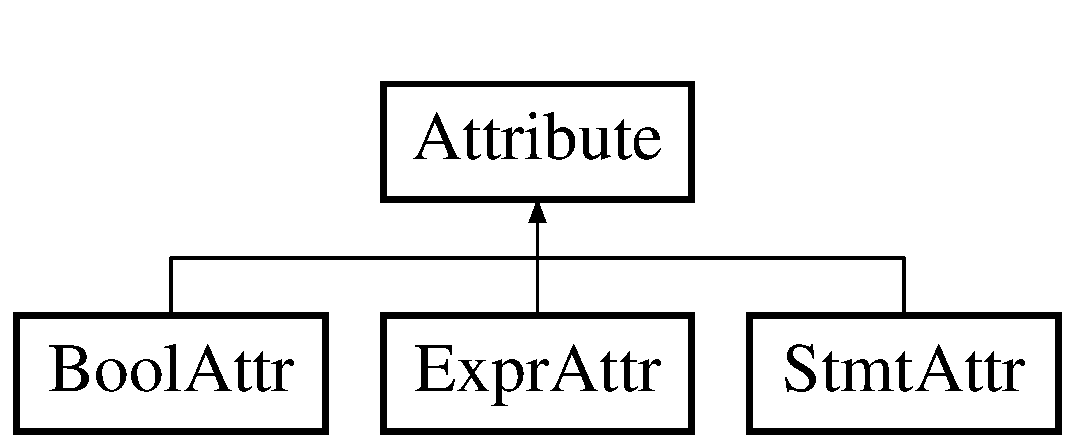
\includegraphics[height=2.000000cm]{class_attribute}
\end{center}
\end{figure}


\subsection{Detailed Description}
An empty class representing the attributes of the grammar symbols. It must be specialized for each specific attribute. 

The documentation for this class was generated from the following file\+:\begin{DoxyCompactItemize}
\item 
\hyperlink{tinycomp_8h}{tinycomp.\+h}\end{DoxyCompactItemize}

\hypertarget{class_bool_attr}{}\section{Bool\+Attr Class Reference}
\label{class_bool_attr}\index{Bool\+Attr@{Bool\+Attr}}


{\ttfamily \#include $<$tinycomp.\+hpp$>$}

Inheritance diagram for Bool\+Attr\+:\begin{figure}[H]
\begin{center}
\leavevmode
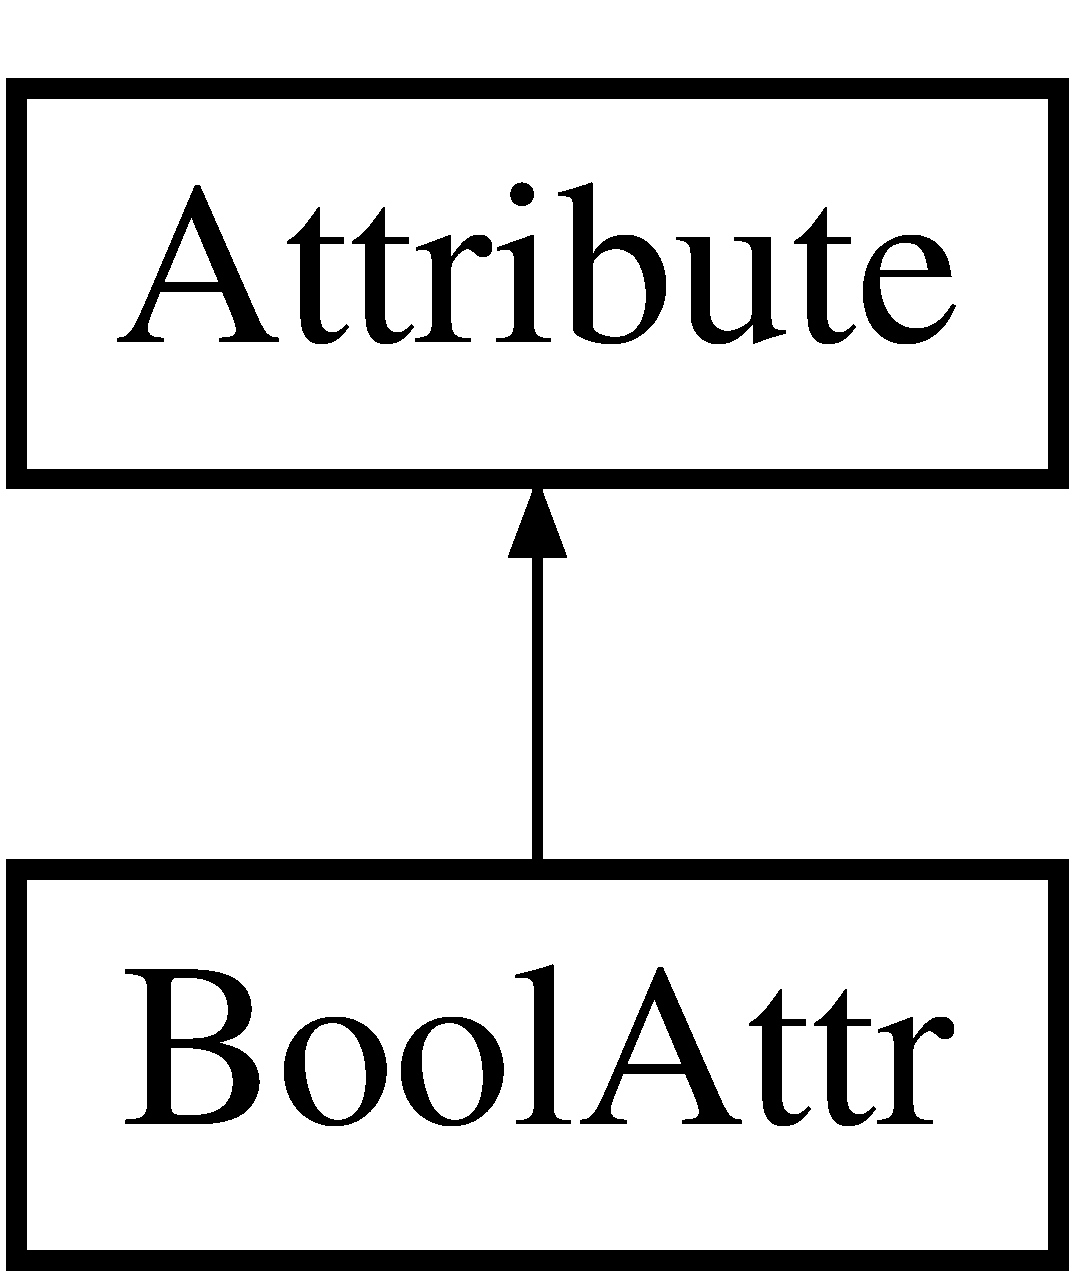
\includegraphics[height=2.000000cm]{class_bool_attr}
\end{center}
\end{figure}
\subsection*{Public Member Functions}
\begin{DoxyCompactItemize}
\item 
void \hyperlink{class_bool_attr_a9437deb583e3b6d353bc4cdc3a3ac003}{add\+True} (\hyperlink{class_tac_instr}{Tac\+Instr} $\ast$instr)
\item 
void \hyperlink{class_bool_attr_aa7a71ac5b804c231b75d060e70d30adc}{add\+False} (\hyperlink{class_tac_instr}{Tac\+Instr} $\ast$instr)
\item 
void \hyperlink{class_bool_attr_acc97b2c9d25818662e8c756d0f804523}{add\+True} (list$<$ \hyperlink{class_tac_instr}{Tac\+Instr} $\ast$ $>$ l)
\item 
void \hyperlink{class_bool_attr_afb2abc67561365b8c7bd1469fa4ff8cd}{add\+False} (list$<$ \hyperlink{class_tac_instr}{Tac\+Instr} $\ast$ $>$ l)
\item 
list$<$ \hyperlink{class_tac_instr}{Tac\+Instr} $\ast$ $>$ \hyperlink{class_bool_attr_aaba8e988b2491bda9cf9f398f53bb0c3}{get\+Truelist} ()
\item 
list$<$ \hyperlink{class_tac_instr}{Tac\+Instr} $\ast$ $>$ \hyperlink{class_bool_attr_a22d66b869b09203424020a5a3c4ceb37}{get\+Falselist} ()
\end{DoxyCompactItemize}


\subsection{Detailed Description}
Implementation of attribute for grammar symbol cond\+: boolean expressions
\begin{DoxyItemize}
\item B.\+truelist
\item B.\+falselist 
\end{DoxyItemize}

\subsection{Member Function Documentation}
\index{Bool\+Attr@{Bool\+Attr}!add\+False@{add\+False}}
\index{add\+False@{add\+False}!Bool\+Attr@{Bool\+Attr}}
\subsubsection[{\texorpdfstring{add\+False(\+Tac\+Instr $\ast$instr)}{addFalse(TacInstr *instr)}}]{\setlength{\rightskip}{0pt plus 5cm}void Bool\+Attr\+::add\+False (
\begin{DoxyParamCaption}
\item[{{\bf Tac\+Instr} $\ast$}]{instr}
\end{DoxyParamCaption}
)}\hypertarget{class_bool_attr_aa7a71ac5b804c231b75d060e70d30adc}{}\label{class_bool_attr_aa7a71ac5b804c231b75d060e70d30adc}
Appends a 3-\/addr code instruction to the falselist.


\begin{DoxyParams}{Parameters}
{\em instr} & The instruction to be appended; it is assumed to contain a \char`\"{}goto\char`\"{}-\/like operator. \\
\hline
\end{DoxyParams}
\index{Bool\+Attr@{Bool\+Attr}!add\+False@{add\+False}}
\index{add\+False@{add\+False}!Bool\+Attr@{Bool\+Attr}}
\subsubsection[{\texorpdfstring{add\+False(list$<$ Tac\+Instr $\ast$ $>$ l)}{addFalse(list< TacInstr * > l)}}]{\setlength{\rightskip}{0pt plus 5cm}void Bool\+Attr\+::add\+False (
\begin{DoxyParamCaption}
\item[{list$<$ {\bf Tac\+Instr} $\ast$ $>$}]{l}
\end{DoxyParamCaption}
)}\hypertarget{class_bool_attr_afb2abc67561365b8c7bd1469fa4ff8cd}{}\label{class_bool_attr_afb2abc67561365b8c7bd1469fa4ff8cd}
Appends a list of instructions to the falselist. Basically, an implementation of merge() for a falselist. 
\begin{DoxyParams}{Parameters}
{\em l} & The list to be appended; it is assumed to contain only \char`\"{}goto\char`\"{}-\/like instructions. \\
\hline
\end{DoxyParams}
\index{Bool\+Attr@{Bool\+Attr}!add\+True@{add\+True}}
\index{add\+True@{add\+True}!Bool\+Attr@{Bool\+Attr}}
\subsubsection[{\texorpdfstring{add\+True(\+Tac\+Instr $\ast$instr)}{addTrue(TacInstr *instr)}}]{\setlength{\rightskip}{0pt plus 5cm}void Bool\+Attr\+::add\+True (
\begin{DoxyParamCaption}
\item[{{\bf Tac\+Instr} $\ast$}]{instr}
\end{DoxyParamCaption}
)}\hypertarget{class_bool_attr_a9437deb583e3b6d353bc4cdc3a3ac003}{}\label{class_bool_attr_a9437deb583e3b6d353bc4cdc3a3ac003}
Appends a 3-\/addr code instruction to the truelist.


\begin{DoxyParams}{Parameters}
{\em instr} & The instruction to be appended; it is assumed to contain a \char`\"{}goto\char`\"{}-\/like operator. \\
\hline
\end{DoxyParams}
\index{Bool\+Attr@{Bool\+Attr}!add\+True@{add\+True}}
\index{add\+True@{add\+True}!Bool\+Attr@{Bool\+Attr}}
\subsubsection[{\texorpdfstring{add\+True(list$<$ Tac\+Instr $\ast$ $>$ l)}{addTrue(list< TacInstr * > l)}}]{\setlength{\rightskip}{0pt plus 5cm}void Bool\+Attr\+::add\+True (
\begin{DoxyParamCaption}
\item[{list$<$ {\bf Tac\+Instr} $\ast$ $>$}]{l}
\end{DoxyParamCaption}
)}\hypertarget{class_bool_attr_acc97b2c9d25818662e8c756d0f804523}{}\label{class_bool_attr_acc97b2c9d25818662e8c756d0f804523}
Appends a list of instructions to the truelist. Basically, an implementation of merge() for a truelist. 
\begin{DoxyParams}{Parameters}
{\em l} & The list to be appended; it is assumed to contain only \char`\"{}goto\char`\"{}-\/like instructions. \\
\hline
\end{DoxyParams}
\index{Bool\+Attr@{Bool\+Attr}!get\+Falselist@{get\+Falselist}}
\index{get\+Falselist@{get\+Falselist}!Bool\+Attr@{Bool\+Attr}}
\subsubsection[{\texorpdfstring{get\+Falselist()}{getFalselist()}}]{\setlength{\rightskip}{0pt plus 5cm}list$<${\bf Tac\+Instr}$\ast$$>$ Bool\+Attr\+::get\+Falselist (
\begin{DoxyParamCaption}
{}
\end{DoxyParamCaption}
)}\hypertarget{class_bool_attr_a22d66b869b09203424020a5a3c4ceb37}{}\label{class_bool_attr_a22d66b869b09203424020a5a3c4ceb37}
Returns the falselist. \index{Bool\+Attr@{Bool\+Attr}!get\+Truelist@{get\+Truelist}}
\index{get\+Truelist@{get\+Truelist}!Bool\+Attr@{Bool\+Attr}}
\subsubsection[{\texorpdfstring{get\+Truelist()}{getTruelist()}}]{\setlength{\rightskip}{0pt plus 5cm}list$<${\bf Tac\+Instr}$\ast$$>$ Bool\+Attr\+::get\+Truelist (
\begin{DoxyParamCaption}
{}
\end{DoxyParamCaption}
)}\hypertarget{class_bool_attr_aaba8e988b2491bda9cf9f398f53bb0c3}{}\label{class_bool_attr_aaba8e988b2491bda9cf9f398f53bb0c3}
Returns the truelist. 

The documentation for this class was generated from the following file\+:\begin{DoxyCompactItemize}
\item 
\hyperlink{tinycomp_8hpp}{tinycomp.\+hpp}\end{DoxyCompactItemize}

\hypertarget{class_const_address}{}\section{Const\+Address Class Reference}
\label{class_const_address}\index{Const\+Address@{Const\+Address}}


{\ttfamily \#include $<$tinycomp.\+hpp$>$}

Inheritance diagram for Const\+Address\+:\begin{figure}[H]
\begin{center}
\leavevmode
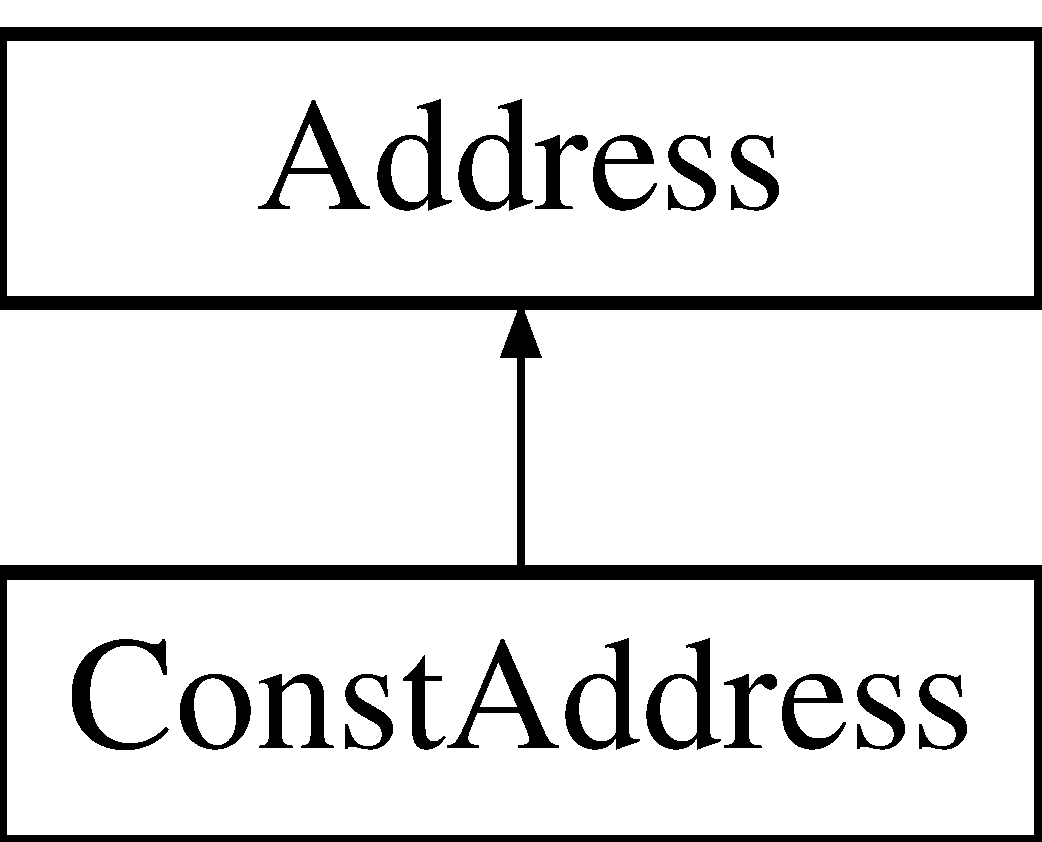
\includegraphics[height=2.000000cm]{class_const_address}
\end{center}
\end{figure}
\subsection*{Public Member Functions}
\begin{DoxyCompactItemize}
\item 
\hyperlink{class_const_address_a3d31b1ad98928a7ab901342651dba352}{Const\+Address} (int i)
\item 
\hyperlink{class_const_address_a7dd2528a30edf7981839455a7817903d}{Const\+Address} (float f)
\item 
\hyperlink{class_const_address_ad8a58bb142ffafd1c375820db95490be}{Const\+Address} (\hyperlink{structfraction}{fraction} f)
\item 
\hyperlink{tinycomp_8h_aca554671f4620139c1393f96d2af74bc}{type\+Name} \hyperlink{class_const_address_a59180f99dc2d75f52c76d3aa2100ab85}{get\+Type} ()
\item 
const char $\ast$ \hyperlink{class_const_address_ae5c661e2c7033c192d493d8345ea6c75}{to\+String} () const 
\end{DoxyCompactItemize}
\subsection*{Additional Inherited Members}


\subsection{Detailed Description}
A specialization of \hyperlink{class_address}{Address} to hold a constant 

\subsection{Constructor \& Destructor Documentation}
\index{Const\+Address@{Const\+Address}!Const\+Address@{Const\+Address}}
\index{Const\+Address@{Const\+Address}!Const\+Address@{Const\+Address}}
\subsubsection[{\texorpdfstring{Const\+Address(int i)}{ConstAddress(int i)}}]{\setlength{\rightskip}{0pt plus 5cm}Const\+Address\+::\+Const\+Address (
\begin{DoxyParamCaption}
\item[{int}]{i}
\end{DoxyParamCaption}
)}\hypertarget{class_const_address_a3d31b1ad98928a7ab901342651dba352}{}\label{class_const_address_a3d31b1ad98928a7ab901342651dba352}
Constructor for an int constant \index{Const\+Address@{Const\+Address}!Const\+Address@{Const\+Address}}
\index{Const\+Address@{Const\+Address}!Const\+Address@{Const\+Address}}
\subsubsection[{\texorpdfstring{Const\+Address(float f)}{ConstAddress(float f)}}]{\setlength{\rightskip}{0pt plus 5cm}Const\+Address\+::\+Const\+Address (
\begin{DoxyParamCaption}
\item[{float}]{f}
\end{DoxyParamCaption}
)}\hypertarget{class_const_address_a7dd2528a30edf7981839455a7817903d}{}\label{class_const_address_a7dd2528a30edf7981839455a7817903d}
Constructor for a float constant. \index{Const\+Address@{Const\+Address}!Const\+Address@{Const\+Address}}
\index{Const\+Address@{Const\+Address}!Const\+Address@{Const\+Address}}
\subsubsection[{\texorpdfstring{Const\+Address(fraction f)}{ConstAddress(fraction f)}}]{\setlength{\rightskip}{0pt plus 5cm}Const\+Address\+::\+Const\+Address (
\begin{DoxyParamCaption}
\item[{{\bf fraction}}]{f}
\end{DoxyParamCaption}
)}\hypertarget{class_const_address_ad8a58bb142ffafd1c375820db95490be}{}\label{class_const_address_ad8a58bb142ffafd1c375820db95490be}
Constructor for fraction constant 

\subsection{Member Function Documentation}
\index{Const\+Address@{Const\+Address}!get\+Type@{get\+Type}}
\index{get\+Type@{get\+Type}!Const\+Address@{Const\+Address}}
\subsubsection[{\texorpdfstring{get\+Type()}{getType()}}]{\setlength{\rightskip}{0pt plus 5cm}{\bf type\+Name} Const\+Address\+::get\+Type (
\begin{DoxyParamCaption}
{}
\end{DoxyParamCaption}
)}\hypertarget{class_const_address_a59180f99dc2d75f52c76d3aa2100ab85}{}\label{class_const_address_a59180f99dc2d75f52c76d3aa2100ab85}
Returns the constant\textquotesingle{}s type (as a type\+Name enum) \index{Const\+Address@{Const\+Address}!to\+String@{to\+String}}
\index{to\+String@{to\+String}!Const\+Address@{Const\+Address}}
\subsubsection[{\texorpdfstring{to\+String() const }{toString() const }}]{\setlength{\rightskip}{0pt plus 5cm}const char$\ast$ Const\+Address\+::to\+String (
\begin{DoxyParamCaption}
{}
\end{DoxyParamCaption}
) const\hspace{0.3cm}{\ttfamily [virtual]}}\hypertarget{class_const_address_ae5c661e2c7033c192d493d8345ea6c75}{}\label{class_const_address_ae5c661e2c7033c192d493d8345ea6c75}
Concrete method for printing a \hyperlink{class_const_address}{Const\+Address}; it\textquotesingle{}s a concrete implementation of the corresponding abstract method in \hyperlink{class_address}{Address} 

Implements \hyperlink{class_address_ac58183c3d3dc7c3e98a17825dd086de1}{Address}.



The documentation for this class was generated from the following file\+:\begin{DoxyCompactItemize}
\item 
\hyperlink{tinycomp_8hpp}{tinycomp.\+hpp}\end{DoxyCompactItemize}

\hypertarget{class_expr_attr}{}\section{Expr\+Attr Class Reference}
\label{class_expr_attr}\index{Expr\+Attr@{Expr\+Attr}}


{\ttfamily \#include $<$tinycomp.\+hpp$>$}

Inheritance diagram for Expr\+Attr\+:\begin{figure}[H]
\begin{center}
\leavevmode
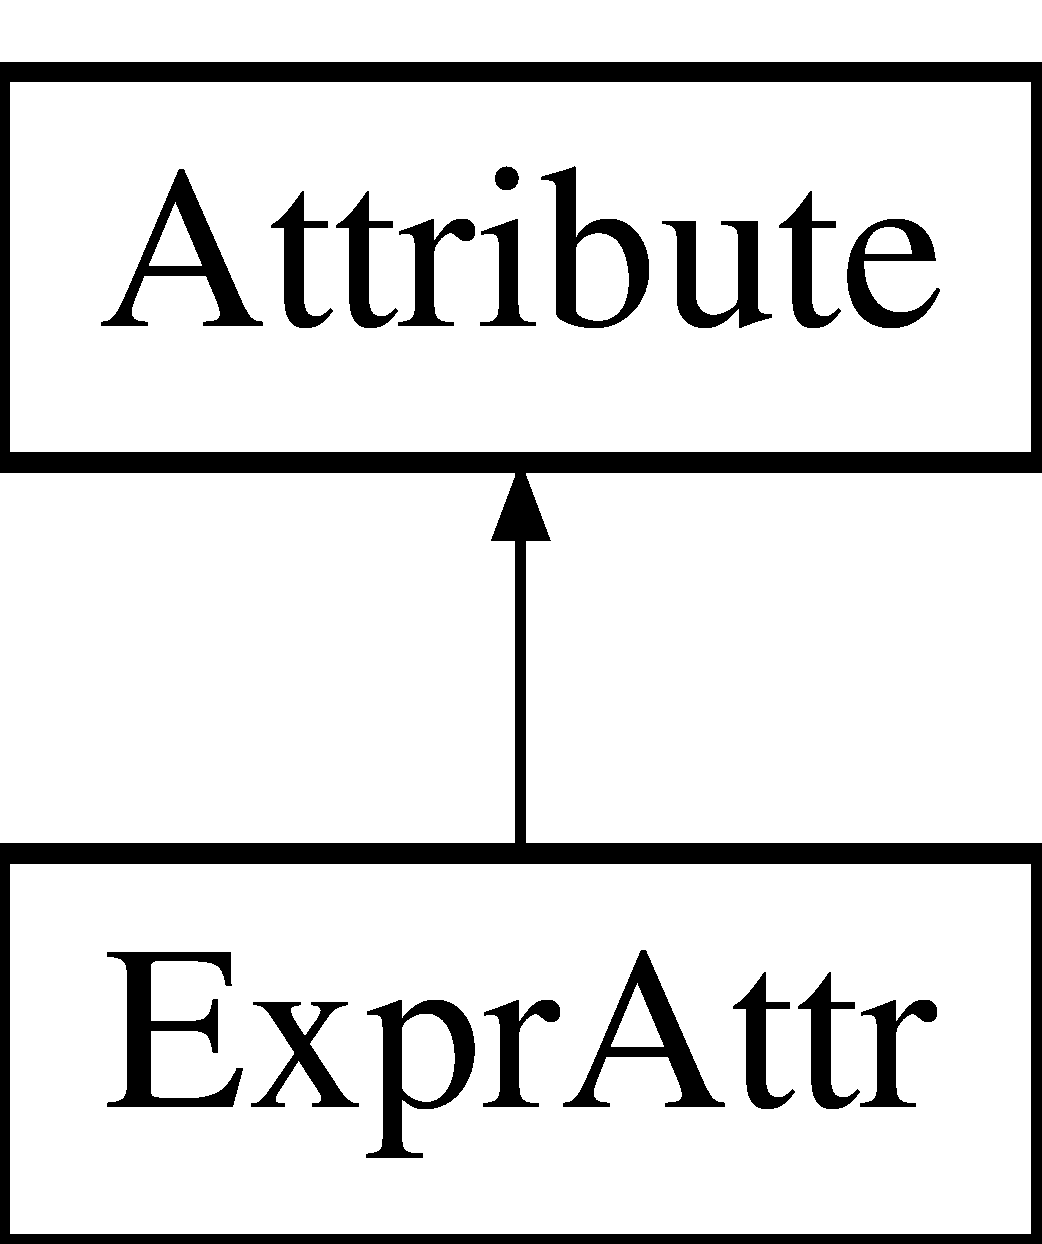
\includegraphics[height=2.000000cm]{class_expr_attr}
\end{center}
\end{figure}
\subsection*{Public Member Functions}
\begin{DoxyCompactItemize}
\item 
\hyperlink{class_expr_attr_a9c7b01b5546a7ad4550915b2004bd10a}{Expr\+Attr} (\hyperlink{class_tac_instr}{Tac\+Instr} $\ast$addr, \hyperlink{tinycomp_8h_aca554671f4620139c1393f96d2af74bc}{type\+Name} type)
\item 
\hyperlink{class_expr_attr_a7362196f3e62587f89134e23b8ee40fc}{Expr\+Attr} (\hyperlink{class_var_address}{Var\+Address} $\ast$addr)
\item 
\hyperlink{class_expr_attr_af2cb2432b6971074b082934a1065aaa0}{Expr\+Attr} (\hyperlink{class_const_address}{Const\+Address} $\ast$addr)
\item 
\hyperlink{class_expr_attr_a61e2a36f551af4024b31c58b1185d7d2}{Expr\+Attr} (\hyperlink{class_temp_address}{Temp\+Address} $\ast$addr, \hyperlink{tinycomp_8h_aca554671f4620139c1393f96d2af74bc}{type\+Name} type)
\item 
\hyperlink{class_address}{Address} $\ast$ \hyperlink{class_expr_attr_aec4263aec2979831b898773b0910bc95}{get\+Addr} ()
\item 
\hyperlink{tinycomp_8h_aca554671f4620139c1393f96d2af74bc}{type\+Name} \hyperlink{class_expr_attr_a17c309d7036192a6d15ebe3388dc0f34}{get\+Type} ()
\end{DoxyCompactItemize}


\subsection{Detailed Description}
Implementation of attribute for grammar symbol expr\+: arithmetic expressions
\begin{DoxyItemize}
\item E.\+addr 
\end{DoxyItemize}

\subsection{Constructor \& Destructor Documentation}
\index{Expr\+Attr@{Expr\+Attr}!Expr\+Attr@{Expr\+Attr}}
\index{Expr\+Attr@{Expr\+Attr}!Expr\+Attr@{Expr\+Attr}}
\subsubsection[{\texorpdfstring{Expr\+Attr(\+Tac\+Instr $\ast$addr, type\+Name type)}{ExprAttr(TacInstr *addr, typeName type)}}]{\setlength{\rightskip}{0pt plus 5cm}Expr\+Attr\+::\+Expr\+Attr (
\begin{DoxyParamCaption}
\item[{{\bf Tac\+Instr} $\ast$}]{addr, }
\item[{{\bf type\+Name}}]{type}
\end{DoxyParamCaption}
)}\hypertarget{class_expr_attr_a9c7b01b5546a7ad4550915b2004bd10a}{}\label{class_expr_attr_a9c7b01b5546a7ad4550915b2004bd10a}
Constructor for \hyperlink{class_expr_attr}{Expr\+Attr}; it will refer to the \hyperlink{class_address}{Address} (valuenumber) of the instruction that (when executed) will contain the result of the entire expression. It needs to know (and store) the type of the result. \index{Expr\+Attr@{Expr\+Attr}!Expr\+Attr@{Expr\+Attr}}
\index{Expr\+Attr@{Expr\+Attr}!Expr\+Attr@{Expr\+Attr}}
\subsubsection[{\texorpdfstring{Expr\+Attr(\+Var\+Address $\ast$addr)}{ExprAttr(VarAddress *addr)}}]{\setlength{\rightskip}{0pt plus 5cm}Expr\+Attr\+::\+Expr\+Attr (
\begin{DoxyParamCaption}
\item[{{\bf Var\+Address} $\ast$}]{addr}
\end{DoxyParamCaption}
)}\hypertarget{class_expr_attr_a7362196f3e62587f89134e23b8ee40fc}{}\label{class_expr_attr_a7362196f3e62587f89134e23b8ee40fc}
Constructor for \hyperlink{class_expr_attr}{Expr\+Attr}; it will refer to the \hyperlink{class_address}{Address} of the variable. It will infer the type from the type of the variable. \index{Expr\+Attr@{Expr\+Attr}!Expr\+Attr@{Expr\+Attr}}
\index{Expr\+Attr@{Expr\+Attr}!Expr\+Attr@{Expr\+Attr}}
\subsubsection[{\texorpdfstring{Expr\+Attr(\+Const\+Address $\ast$addr)}{ExprAttr(ConstAddress *addr)}}]{\setlength{\rightskip}{0pt plus 5cm}Expr\+Attr\+::\+Expr\+Attr (
\begin{DoxyParamCaption}
\item[{{\bf Const\+Address} $\ast$}]{addr}
\end{DoxyParamCaption}
)}\hypertarget{class_expr_attr_af2cb2432b6971074b082934a1065aaa0}{}\label{class_expr_attr_af2cb2432b6971074b082934a1065aaa0}
Constructor for \hyperlink{class_expr_attr}{Expr\+Attr}; it will refer to a constant. It will infer the type from the type of the constant. \index{Expr\+Attr@{Expr\+Attr}!Expr\+Attr@{Expr\+Attr}}
\index{Expr\+Attr@{Expr\+Attr}!Expr\+Attr@{Expr\+Attr}}
\subsubsection[{\texorpdfstring{Expr\+Attr(\+Temp\+Address $\ast$addr, type\+Name type)}{ExprAttr(TempAddress *addr, typeName type)}}]{\setlength{\rightskip}{0pt plus 5cm}Expr\+Attr\+::\+Expr\+Attr (
\begin{DoxyParamCaption}
\item[{{\bf Temp\+Address} $\ast$}]{addr, }
\item[{{\bf type\+Name}}]{type}
\end{DoxyParamCaption}
)}\hypertarget{class_expr_attr_a61e2a36f551af4024b31c58b1185d7d2}{}\label{class_expr_attr_a61e2a36f551af4024b31c58b1185d7d2}
Constructor for \hyperlink{class_expr_attr}{Expr\+Attr}; it will refer to a temporary, supposedly holding some variable. The type cannot be inferred, in ths case, so it must be explicitly provided. 

\subsection{Member Function Documentation}
\index{Expr\+Attr@{Expr\+Attr}!get\+Addr@{get\+Addr}}
\index{get\+Addr@{get\+Addr}!Expr\+Attr@{Expr\+Attr}}
\subsubsection[{\texorpdfstring{get\+Addr()}{getAddr()}}]{\setlength{\rightskip}{0pt plus 5cm}{\bf Address}$\ast$ Expr\+Attr\+::get\+Addr (
\begin{DoxyParamCaption}
{}
\end{DoxyParamCaption}
)}\hypertarget{class_expr_attr_aec4263aec2979831b898773b0910bc95}{}\label{class_expr_attr_aec4263aec2979831b898773b0910bc95}
Returns the E.\+addr attribute \index{Expr\+Attr@{Expr\+Attr}!get\+Type@{get\+Type}}
\index{get\+Type@{get\+Type}!Expr\+Attr@{Expr\+Attr}}
\subsubsection[{\texorpdfstring{get\+Type()}{getType()}}]{\setlength{\rightskip}{0pt plus 5cm}{\bf type\+Name} Expr\+Attr\+::get\+Type (
\begin{DoxyParamCaption}
{}
\end{DoxyParamCaption}
)}\hypertarget{class_expr_attr_a17c309d7036192a6d15ebe3388dc0f34}{}\label{class_expr_attr_a17c309d7036192a6d15ebe3388dc0f34}
Returns the E.\+type attribute 

The documentation for this class was generated from the following file\+:\begin{DoxyCompactItemize}
\item 
\hyperlink{tinycomp_8hpp}{tinycomp.\+hpp}\end{DoxyCompactItemize}

\hypertarget{structfraction}{}\section{fraction Struct Reference}
\label{structfraction}\index{fraction@{fraction}}


{\ttfamily \#include $<$tinycomp.\+h$>$}

\subsection*{Data Fields}
\begin{DoxyCompactItemize}
\item 
int \hyperlink{structfraction_a7700ec3a4dbbd05ba26e243fe5583a85}{num}
\item 
int \hyperlink{structfraction_ae34d45953c8a4d73737d223de22e18c3}{denom}
\end{DoxyCompactItemize}


\subsection{Detailed Description}
Structure for holding fraction type 

\subsection{Field Documentation}
\index{fraction@{fraction}!denom@{denom}}
\index{denom@{denom}!fraction@{fraction}}
\subsubsection[{\texorpdfstring{denom}{denom}}]{\setlength{\rightskip}{0pt plus 5cm}int fraction\+::denom}\hypertarget{structfraction_ae34d45953c8a4d73737d223de22e18c3}{}\label{structfraction_ae34d45953c8a4d73737d223de22e18c3}
denominator value \index{fraction@{fraction}!num@{num}}
\index{num@{num}!fraction@{fraction}}
\subsubsection[{\texorpdfstring{num}{num}}]{\setlength{\rightskip}{0pt plus 5cm}int fraction\+::num}\hypertarget{structfraction_a7700ec3a4dbbd05ba26e243fe5583a85}{}\label{structfraction_a7700ec3a4dbbd05ba26e243fe5583a85}
numerator value 

The documentation for this struct was generated from the following file\+:\begin{DoxyCompactItemize}
\item 
\hyperlink{tinycomp_8h}{tinycomp.\+h}\end{DoxyCompactItemize}

\hypertarget{class_instr_address}{}\section{Instr\+Address Class Reference}
\label{class_instr_address}\index{Instr\+Address@{Instr\+Address}}


{\ttfamily \#include $<$tinycomp.\+hpp$>$}

Inheritance diagram for Instr\+Address\+:\begin{figure}[H]
\begin{center}
\leavevmode
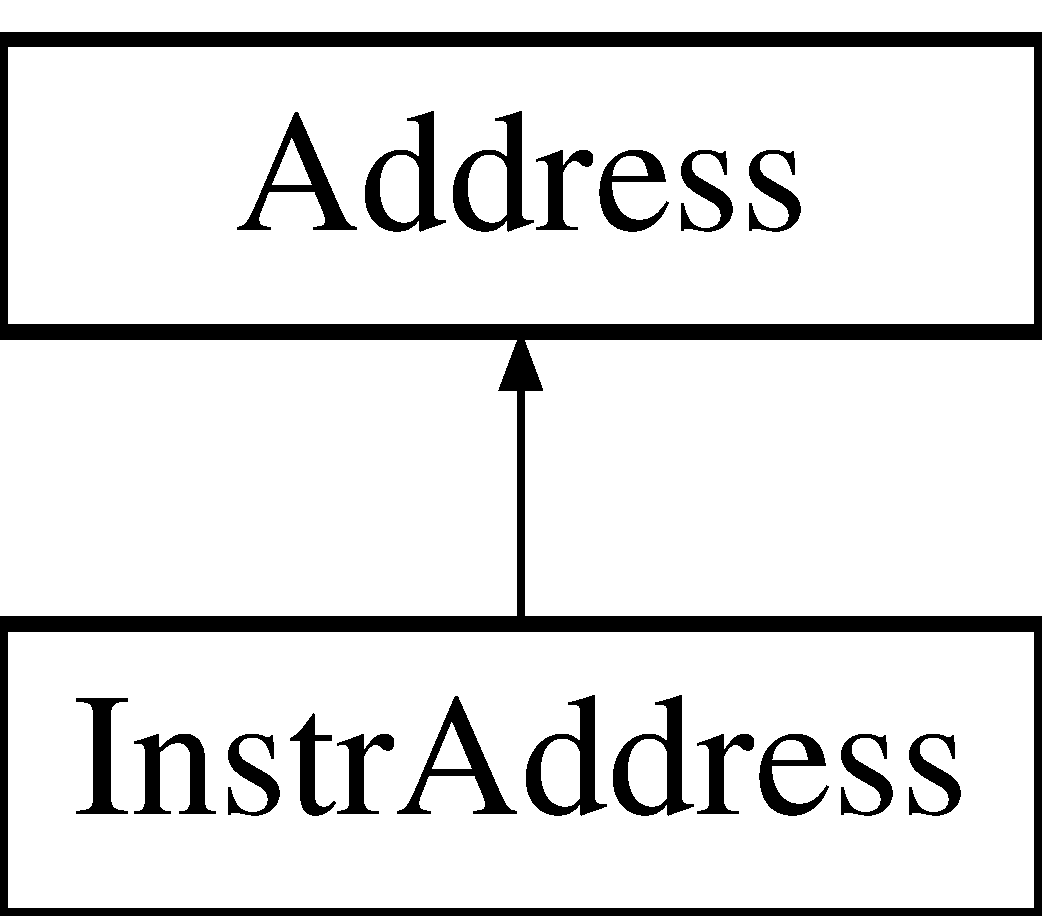
\includegraphics[height=2.000000cm]{class_instr_address}
\end{center}
\end{figure}
\subsection*{Public Member Functions}
\begin{DoxyCompactItemize}
\item 
\hyperlink{class_instr_address_a966c221ee738631ef72bdf7d2bcb2771}{Instr\+Address} (int vn)
\item 
const char $\ast$ \hyperlink{class_instr_address_a4cf3f82f491d6bc401008d93ced13b17}{to\+String} () const 
\end{DoxyCompactItemize}
\subsection*{Friends}
\begin{DoxyCompactItemize}
\item 
std\+::ostream \& {\bfseries operator$<$$<$} (std\+::ostream \&, const \hyperlink{class_instr_address}{Instr\+Address} $\ast$)\hypertarget{class_instr_address_aa218b6426f449d15a282b4ba5d3c07c3}{}\label{class_instr_address_aa218b6426f449d15a282b4ba5d3c07c3}

\end{DoxyCompactItemize}
\subsection*{Additional Inherited Members}


\subsection{Detailed Description}
A specialization of \hyperlink{class_address}{Address} to hold an instruction. 

\subsection{Constructor \& Destructor Documentation}
\index{Instr\+Address@{Instr\+Address}!Instr\+Address@{Instr\+Address}}
\index{Instr\+Address@{Instr\+Address}!Instr\+Address@{Instr\+Address}}
\subsubsection[{\texorpdfstring{Instr\+Address(int vn)}{InstrAddress(int vn)}}]{\setlength{\rightskip}{0pt plus 5cm}Instr\+Address\+::\+Instr\+Address (
\begin{DoxyParamCaption}
\item[{int}]{vn}
\end{DoxyParamCaption}
)}\hypertarget{class_instr_address_a966c221ee738631ef72bdf7d2bcb2771}{}\label{class_instr_address_a966c221ee738631ef72bdf7d2bcb2771}
Constructor to initialize an \hyperlink{class_instr_address}{Instr\+Address} from an index of the array code. 
\begin{DoxyParams}{Parameters}
{\em vn} & The index of the \hyperlink{class_target_code}{Target\+Code} array, representing a valuenumber. \\
\hline
\end{DoxyParams}


\subsection{Member Function Documentation}
\index{Instr\+Address@{Instr\+Address}!to\+String@{to\+String}}
\index{to\+String@{to\+String}!Instr\+Address@{Instr\+Address}}
\subsubsection[{\texorpdfstring{to\+String() const }{toString() const }}]{\setlength{\rightskip}{0pt plus 5cm}const char$\ast$ Instr\+Address\+::to\+String (
\begin{DoxyParamCaption}
{}
\end{DoxyParamCaption}
) const\hspace{0.3cm}{\ttfamily [virtual]}}\hypertarget{class_instr_address_a4cf3f82f491d6bc401008d93ced13b17}{}\label{class_instr_address_a4cf3f82f491d6bc401008d93ced13b17}
Abstract method for printing an \hyperlink{class_address}{Address}. Note that \hyperlink{class_instr_address_a4cf3f82f491d6bc401008d93ced13b17}{to\+String()} {\itshape must} be defined in derived classes. 

Implements \hyperlink{class_address_ac58183c3d3dc7c3e98a17825dd086de1}{Address}.



The documentation for this class was generated from the following file\+:\begin{DoxyCompactItemize}
\item 
\hyperlink{tinycomp_8hpp}{tinycomp.\+hpp}\end{DoxyCompactItemize}

\hypertarget{class_memory}{}\section{Memory Class Reference}
\label{class_memory}\index{Memory@{Memory}}


{\ttfamily \#include $<$tinycomp.\+hpp$>$}

\subsection*{Public Member Functions}
\begin{DoxyCompactItemize}
\item 
int \hyperlink{class_memory_ab07133625f6fc3ef7e094768896ed2fb}{store} (void $\ast$val, int width)
\item 
void $\ast$ \hyperlink{class_memory_afbe4f8f6d315e8663a164eb2c44b2def}{retrieve} (int offset)
\item 
\hyperlink{class_temp_address}{Temp\+Address} $\ast$ \hyperlink{class_memory_ad04d1a36f88c219d7447c10c098e4530}{get\+New\+Temp} (int width)
\item 
void \hyperlink{class_memory_a49ce489fcc012c09284dcc8c1bc4d52b}{hexdump} ()
\item 
void \hyperlink{class_memory_a2f0418e16871271c242acf67894ffa1c}{print\+Out} (\hyperlink{class_sym_tbl}{Sym\+Tbl} $\ast$tbl)
\end{DoxyCompactItemize}
\subsection*{Static Public Member Functions}
\begin{DoxyCompactItemize}
\item 
static \hyperlink{class_memory}{Memory} \& \hyperlink{class_memory_a96eac3970b3baba973645a9cc32aee4c}{get\+Instance} ()
\end{DoxyCompactItemize}
\subsection*{Static Public Attributes}
\begin{DoxyCompactItemize}
\item 
static const int \hyperlink{class_memory_a1f45f0eb9259f5c73cdbb1190212315f}{M\+E\+M\+S\+I\+ZE} = 128
\end{DoxyCompactItemize}


\subsection{Detailed Description}
A simplified abstraction for the memory allocated to the compiler. 

\subsection{Member Function Documentation}
\index{Memory@{Memory}!get\+Instance@{get\+Instance}}
\index{get\+Instance@{get\+Instance}!Memory@{Memory}}
\subsubsection[{\texorpdfstring{get\+Instance()}{getInstance()}}]{\setlength{\rightskip}{0pt plus 5cm}static {\bf Memory}\& Memory\+::get\+Instance (
\begin{DoxyParamCaption}
{}
\end{DoxyParamCaption}
)\hspace{0.3cm}{\ttfamily [static]}}\hypertarget{class_memory_a96eac3970b3baba973645a9cc32aee4c}{}\label{class_memory_a96eac3970b3baba973645a9cc32aee4c}
As \hyperlink{class_memory}{Memory} is implemented as a singleton, its constructor is private. This method is the only way to obtain an instance of \hyperlink{class_memory}{Memory}. It is guaranteed that it will return always the same instance. \index{Memory@{Memory}!get\+New\+Temp@{get\+New\+Temp}}
\index{get\+New\+Temp@{get\+New\+Temp}!Memory@{Memory}}
\subsubsection[{\texorpdfstring{get\+New\+Temp(int width)}{getNewTemp(int width)}}]{\setlength{\rightskip}{0pt plus 5cm}{\bf Temp\+Address}$\ast$ Memory\+::get\+New\+Temp (
\begin{DoxyParamCaption}
\item[{int}]{width}
\end{DoxyParamCaption}
)}\hypertarget{class_memory_ad04d1a36f88c219d7447c10c098e4530}{}\label{class_memory_ad04d1a36f88c219d7447c10c098e4530}
Returns a new temporary address pointing to the first location of available memory Since we would later need to advance the offset anyway, this methods takes care of this; that\textquotesingle{}s why we pass the width of what we\textquotesingle{}re gonna store in that location.

It returns the {\itshape beginning} address of the value to be stored therein (i.\+e. the address of the temporary) \index{Memory@{Memory}!hexdump@{hexdump}}
\index{hexdump@{hexdump}!Memory@{Memory}}
\subsubsection[{\texorpdfstring{hexdump()}{hexdump()}}]{\setlength{\rightskip}{0pt plus 5cm}void Memory\+::hexdump (
\begin{DoxyParamCaption}
{}
\end{DoxyParamCaption}
)}\hypertarget{class_memory_a49ce489fcc012c09284dcc8c1bc4d52b}{}\label{class_memory_a49ce489fcc012c09284dcc8c1bc4d52b}
Prints out a dump of the memory. It prints the content of each memory location in hex format. Not very useful for you, since the memory will be filled only at runtime, but included for completeness. \index{Memory@{Memory}!print\+Out@{print\+Out}}
\index{print\+Out@{print\+Out}!Memory@{Memory}}
\subsubsection[{\texorpdfstring{print\+Out(\+Sym\+Tbl $\ast$tbl)}{printOut(SymTbl *tbl)}}]{\setlength{\rightskip}{0pt plus 5cm}void Memory\+::print\+Out (
\begin{DoxyParamCaption}
\item[{{\bf Sym\+Tbl} $\ast$}]{tbl}
\end{DoxyParamCaption}
)}\hypertarget{class_memory_a2f0418e16871271c242acf67894ffa1c}{}\label{class_memory_a2f0418e16871271c242acf67894ffa1c}
Prints out a logical view of the memory \index{Memory@{Memory}!retrieve@{retrieve}}
\index{retrieve@{retrieve}!Memory@{Memory}}
\subsubsection[{\texorpdfstring{retrieve(int offset)}{retrieve(int offset)}}]{\setlength{\rightskip}{0pt plus 5cm}void$\ast$ Memory\+::retrieve (
\begin{DoxyParamCaption}
\item[{int}]{offset}
\end{DoxyParamCaption}
)}\hypertarget{class_memory_afbe4f8f6d315e8663a164eb2c44b2def}{}\label{class_memory_afbe4f8f6d315e8663a164eb2c44b2def}
Returns the {\itshape beginning} address of some value, supposedly stored in memory. Note that we have no clue about the type of such value, or it\textquotesingle{}s width. They must be \char`\"{}computed/retrieved\char`\"{} externally. \index{Memory@{Memory}!store@{store}}
\index{store@{store}!Memory@{Memory}}
\subsubsection[{\texorpdfstring{store(void $\ast$val, int width)}{store(void *val, int width)}}]{\setlength{\rightskip}{0pt plus 5cm}int Memory\+::store (
\begin{DoxyParamCaption}
\item[{void $\ast$}]{val, }
\item[{int}]{width}
\end{DoxyParamCaption}
)}\hypertarget{class_memory_ab07133625f6fc3ef7e094768896ed2fb}{}\label{class_memory_ab07133625f6fc3ef7e094768896ed2fb}
Store the bytes pointed to by val in memory. Note that we don\textquotesingle{}t pass the type of the variable to be stored, as this has no relevance for the memory.

Returns the {\itshape beginning} address of the value just stored. 

\subsection{Field Documentation}
\index{Memory@{Memory}!M\+E\+M\+S\+I\+ZE@{M\+E\+M\+S\+I\+ZE}}
\index{M\+E\+M\+S\+I\+ZE@{M\+E\+M\+S\+I\+ZE}!Memory@{Memory}}
\subsubsection[{\texorpdfstring{M\+E\+M\+S\+I\+ZE}{MEMSIZE}}]{\setlength{\rightskip}{0pt plus 5cm}const int Memory\+::\+M\+E\+M\+S\+I\+ZE = 128\hspace{0.3cm}{\ttfamily [static]}}\hypertarget{class_memory_a1f45f0eb9259f5c73cdbb1190212315f}{}\label{class_memory_a1f45f0eb9259f5c73cdbb1190212315f}
The size of our memory in bytes. It\textquotesingle{}s set to a very small value to keep visualization of the memory dump clean. Increase as needed. 

The documentation for this class was generated from the following file\+:\begin{DoxyCompactItemize}
\item 
\hyperlink{tinycomp_8hpp}{tinycomp.\+hpp}\end{DoxyCompactItemize}

\hypertarget{class_simple_array_sym_tbl}{}\section{Simple\+Array\+Sym\+Tbl Class Reference}
\label{class_simple_array_sym_tbl}\index{Simple\+Array\+Sym\+Tbl@{Simple\+Array\+Sym\+Tbl}}


{\ttfamily \#include $<$tinycomp.\+hpp$>$}

Inheritance diagram for Simple\+Array\+Sym\+Tbl\+:\begin{figure}[H]
\begin{center}
\leavevmode
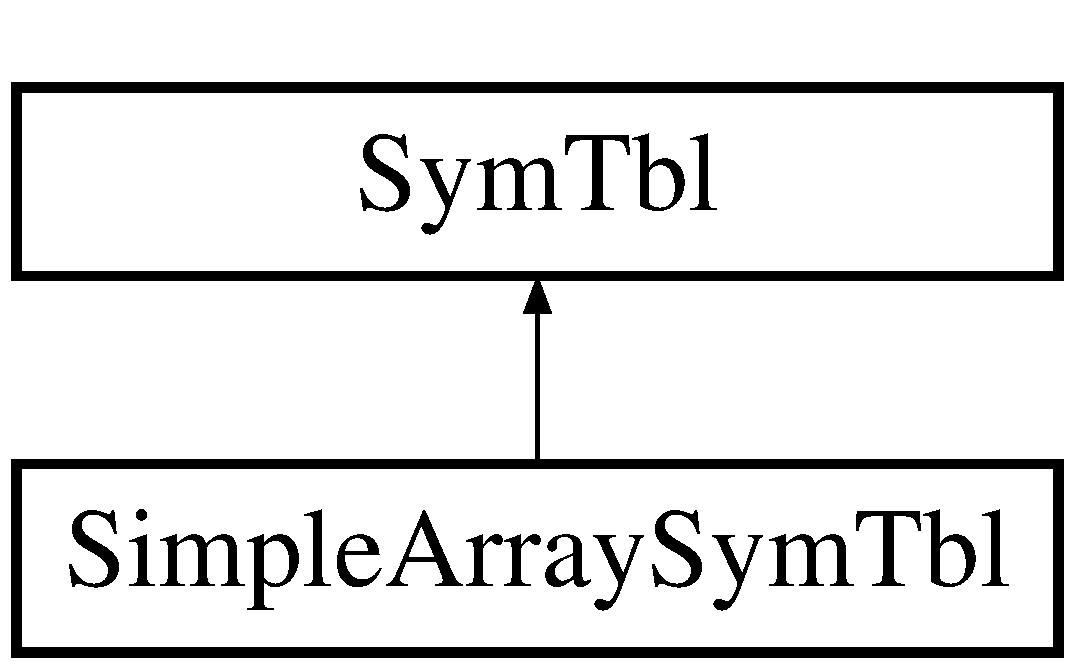
\includegraphics[height=2.000000cm]{class_simple_array_sym_tbl}
\end{center}
\end{figure}
\subsection*{Public Member Functions}
\begin{DoxyCompactItemize}
\item 
\hyperlink{class_simple_array_sym_tbl_a66b279785f28f0aefbaa0230792ef94a}{Simple\+Array\+Sym\+Tbl} ()
\item 
\hyperlink{class_var_address}{Var\+Address} $\ast$ \hyperlink{class_simple_array_sym_tbl_a28d6d5c513f7b8f2beee3a0cf6eab45b}{get} (const char $\ast$lexeme)
\item 
\hyperlink{class_var_address}{Var\+Address} $\ast$ \hyperlink{class_simple_array_sym_tbl_a56a8105f91e5436d8396ed57a374ed5f}{get} (char lexeme)
\item 
void \hyperlink{class_simple_array_sym_tbl_ac7a485531efeaf7b6ac6b5215e212a37}{put} (const char $\ast$lexeme, \hyperlink{tinycomp_8h_aca554671f4620139c1393f96d2af74bc}{type\+Name} type)
\item 
void \hyperlink{class_simple_array_sym_tbl_a12e8b965e1d43cf9b037c262d0400295}{put} (char lexeme, \hyperlink{tinycomp_8h_aca554671f4620139c1393f96d2af74bc}{type\+Name} type)
\item 
void $\ast$ \hyperlink{class_simple_array_sym_tbl_a2f8a29297406612782319c8b069ce17a}{get\+Var\+Value} (char lexeme)
\item 
void \hyperlink{class_simple_array_sym_tbl_aa96c422e9a48887d1756d1b13d2f41d3}{print\+Out} ()
\item 
void \hyperlink{class_simple_array_sym_tbl_af761f997d593f4da432a8ba448b4fae2}{print\+Memory} ()
\end{DoxyCompactItemize}
\subsection*{Additional Inherited Members}


\subsection{Detailed Description}
A simple implementation for a symbol table. I assume here that var id\textquotesingle{}s are 1-\/char long, so the table is just an array with 26 entries. 

\subsection{Constructor \& Destructor Documentation}
\index{Simple\+Array\+Sym\+Tbl@{Simple\+Array\+Sym\+Tbl}!Simple\+Array\+Sym\+Tbl@{Simple\+Array\+Sym\+Tbl}}
\index{Simple\+Array\+Sym\+Tbl@{Simple\+Array\+Sym\+Tbl}!Simple\+Array\+Sym\+Tbl@{Simple\+Array\+Sym\+Tbl}}
\subsubsection[{\texorpdfstring{Simple\+Array\+Sym\+Tbl()}{SimpleArraySymTbl()}}]{\setlength{\rightskip}{0pt plus 5cm}Simple\+Array\+Sym\+Tbl\+::\+Simple\+Array\+Sym\+Tbl (
\begin{DoxyParamCaption}
{}
\end{DoxyParamCaption}
)}\hypertarget{class_simple_array_sym_tbl_a66b279785f28f0aefbaa0230792ef94a}{}\label{class_simple_array_sym_tbl_a66b279785f28f0aefbaa0230792ef94a}
Constructor for the \hyperlink{class_simple_array_sym_tbl}{Simple\+Array\+Sym\+Tbl} class Basically, it just initializes all entries in the table to N\+U\+LL 

\subsection{Member Function Documentation}
\index{Simple\+Array\+Sym\+Tbl@{Simple\+Array\+Sym\+Tbl}!get@{get}}
\index{get@{get}!Simple\+Array\+Sym\+Tbl@{Simple\+Array\+Sym\+Tbl}}
\subsubsection[{\texorpdfstring{get(const char $\ast$lexeme)}{get(const char *lexeme)}}]{\setlength{\rightskip}{0pt plus 5cm}{\bf Var\+Address}$\ast$ Simple\+Array\+Sym\+Tbl\+::get (
\begin{DoxyParamCaption}
\item[{const char $\ast$}]{lexeme}
\end{DoxyParamCaption}
)\hspace{0.3cm}{\ttfamily [virtual]}}\hypertarget{class_simple_array_sym_tbl_a28d6d5c513f7b8f2beee3a0cf6eab45b}{}\label{class_simple_array_sym_tbl_a28d6d5c513f7b8f2beee3a0cf6eab45b}
Returns an entry, indexed by its lexeme 

Implements \hyperlink{class_sym_tbl_a7cdd50cd38f3eecf23c9e6ce0c1696da}{Sym\+Tbl}.

\index{Simple\+Array\+Sym\+Tbl@{Simple\+Array\+Sym\+Tbl}!get@{get}}
\index{get@{get}!Simple\+Array\+Sym\+Tbl@{Simple\+Array\+Sym\+Tbl}}
\subsubsection[{\texorpdfstring{get(char lexeme)}{get(char lexeme)}}]{\setlength{\rightskip}{0pt plus 5cm}{\bf Var\+Address}$\ast$ Simple\+Array\+Sym\+Tbl\+::get (
\begin{DoxyParamCaption}
\item[{char}]{lexeme}
\end{DoxyParamCaption}
)}\hypertarget{class_simple_array_sym_tbl_a56a8105f91e5436d8396ed57a374ed5f}{}\label{class_simple_array_sym_tbl_a56a8105f91e5436d8396ed57a374ed5f}
Returns an entry, indexed by its lexeme (1-\/char version) \index{Simple\+Array\+Sym\+Tbl@{Simple\+Array\+Sym\+Tbl}!get\+Var\+Value@{get\+Var\+Value}}
\index{get\+Var\+Value@{get\+Var\+Value}!Simple\+Array\+Sym\+Tbl@{Simple\+Array\+Sym\+Tbl}}
\subsubsection[{\texorpdfstring{get\+Var\+Value(char lexeme)}{getVarValue(char lexeme)}}]{\setlength{\rightskip}{0pt plus 5cm}void$\ast$ Simple\+Array\+Sym\+Tbl\+::get\+Var\+Value (
\begin{DoxyParamCaption}
\item[{char}]{lexeme}
\end{DoxyParamCaption}
)\hspace{0.3cm}{\ttfamily [inline]}}\hypertarget{class_simple_array_sym_tbl_a2f8a29297406612782319c8b069ce17a}{}\label{class_simple_array_sym_tbl_a2f8a29297406612782319c8b069ce17a}
Returns the value of a variable by first recovering the offset, and then accessing the memory. Since we don\textquotesingle{}t know the type to be returned, a (void$\ast$) is used. \index{Simple\+Array\+Sym\+Tbl@{Simple\+Array\+Sym\+Tbl}!print\+Memory@{print\+Memory}}
\index{print\+Memory@{print\+Memory}!Simple\+Array\+Sym\+Tbl@{Simple\+Array\+Sym\+Tbl}}
\subsubsection[{\texorpdfstring{print\+Memory()}{printMemory()}}]{\setlength{\rightskip}{0pt plus 5cm}void Simple\+Array\+Sym\+Tbl\+::print\+Memory (
\begin{DoxyParamCaption}
{}
\end{DoxyParamCaption}
)}\hypertarget{class_simple_array_sym_tbl_af761f997d593f4da432a8ba448b4fae2}{}\label{class_simple_array_sym_tbl_af761f997d593f4da432a8ba448b4fae2}
Prints out a logical view of the memory \index{Simple\+Array\+Sym\+Tbl@{Simple\+Array\+Sym\+Tbl}!print\+Out@{print\+Out}}
\index{print\+Out@{print\+Out}!Simple\+Array\+Sym\+Tbl@{Simple\+Array\+Sym\+Tbl}}
\subsubsection[{\texorpdfstring{print\+Out()}{printOut()}}]{\setlength{\rightskip}{0pt plus 5cm}void Simple\+Array\+Sym\+Tbl\+::print\+Out (
\begin{DoxyParamCaption}
{}
\end{DoxyParamCaption}
)}\hypertarget{class_simple_array_sym_tbl_aa96c422e9a48887d1756d1b13d2f41d3}{}\label{class_simple_array_sym_tbl_aa96c422e9a48887d1756d1b13d2f41d3}
Prints out the symbl table \index{Simple\+Array\+Sym\+Tbl@{Simple\+Array\+Sym\+Tbl}!put@{put}}
\index{put@{put}!Simple\+Array\+Sym\+Tbl@{Simple\+Array\+Sym\+Tbl}}
\subsubsection[{\texorpdfstring{put(const char $\ast$lexeme, type\+Name type)}{put(const char *lexeme, typeName type)}}]{\setlength{\rightskip}{0pt plus 5cm}void Simple\+Array\+Sym\+Tbl\+::put (
\begin{DoxyParamCaption}
\item[{const char $\ast$}]{lexeme, }
\item[{{\bf type\+Name}}]{type}
\end{DoxyParamCaption}
)\hspace{0.3cm}{\ttfamily [virtual]}}\hypertarget{class_simple_array_sym_tbl_ac7a485531efeaf7b6ac6b5215e212a37}{}\label{class_simple_array_sym_tbl_ac7a485531efeaf7b6ac6b5215e212a37}
Stores a variable in the symbol table, given its lexeme and type 

Implements \hyperlink{class_sym_tbl_a116640842b4776c1bacc6292b3015078}{Sym\+Tbl}.

\index{Simple\+Array\+Sym\+Tbl@{Simple\+Array\+Sym\+Tbl}!put@{put}}
\index{put@{put}!Simple\+Array\+Sym\+Tbl@{Simple\+Array\+Sym\+Tbl}}
\subsubsection[{\texorpdfstring{put(char lexeme, type\+Name type)}{put(char lexeme, typeName type)}}]{\setlength{\rightskip}{0pt plus 5cm}void Simple\+Array\+Sym\+Tbl\+::put (
\begin{DoxyParamCaption}
\item[{char}]{lexeme, }
\item[{{\bf type\+Name}}]{type}
\end{DoxyParamCaption}
)}\hypertarget{class_simple_array_sym_tbl_a12e8b965e1d43cf9b037c262d0400295}{}\label{class_simple_array_sym_tbl_a12e8b965e1d43cf9b037c262d0400295}
Stores a variable in the symbol table, given its lexeme (1-\/char version) and type 

The documentation for this class was generated from the following file\+:\begin{DoxyCompactItemize}
\item 
\hyperlink{tinycomp_8hpp}{tinycomp.\+hpp}\end{DoxyCompactItemize}

\hypertarget{class_stmt_attr}{}\section{Stmt\+Attr Class Reference}
\label{class_stmt_attr}\index{Stmt\+Attr@{Stmt\+Attr}}


{\ttfamily \#include $<$tinycomp.\+hpp$>$}

Inheritance diagram for Stmt\+Attr\+:\begin{figure}[H]
\begin{center}
\leavevmode
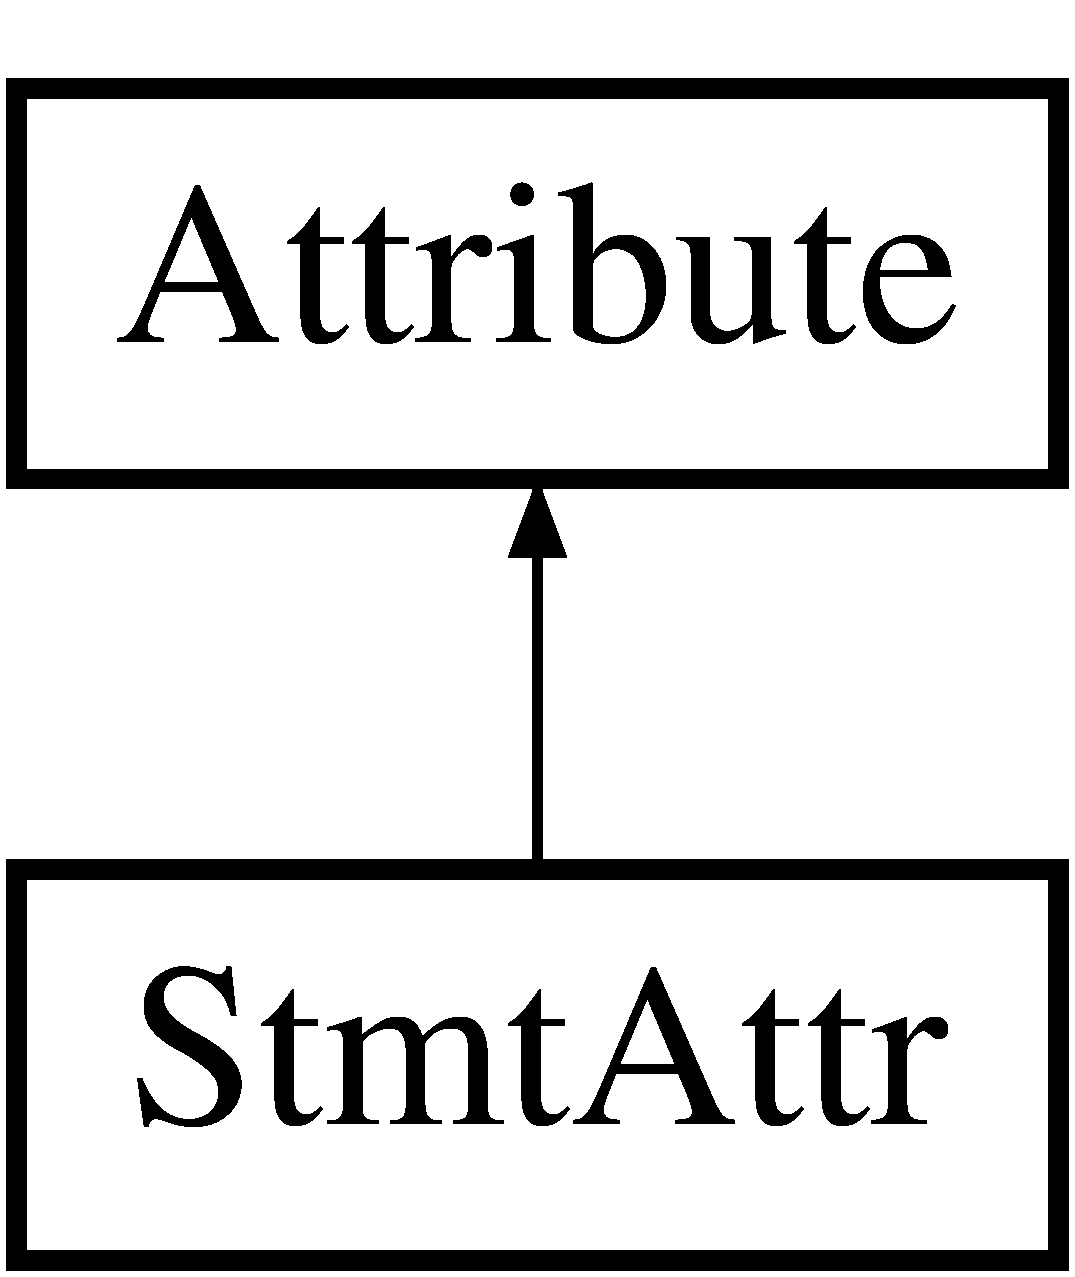
\includegraphics[height=2.000000cm]{class_stmt_attr}
\end{center}
\end{figure}
\subsection*{Public Member Functions}
\begin{DoxyCompactItemize}
\item 
void \hyperlink{class_stmt_attr_aa033b133103d91245cd078b95803f398}{add\+Next} (\hyperlink{class_tac_instr}{Tac\+Instr} $\ast$)
\item 
void \hyperlink{class_stmt_attr_a75a9fbaf6c796c0a42a9b6be18c7bb58}{add\+Next} (list$<$ \hyperlink{class_tac_instr}{Tac\+Instr} $\ast$ $>$ l)
\item 
list$<$ \hyperlink{class_tac_instr}{Tac\+Instr} $\ast$ $>$ \hyperlink{class_stmt_attr_aa76b432ceb444453f8d4386cfb6ea1f0}{get\+Nextlist} ()
\end{DoxyCompactItemize}


\subsection{Detailed Description}
Implementation of attribute for grammar symbol stmt\+: a generic statement.
\begin{DoxyItemize}
\item S.\+nextlist 
\end{DoxyItemize}

\subsection{Member Function Documentation}
\index{Stmt\+Attr@{Stmt\+Attr}!add\+Next@{add\+Next}}
\index{add\+Next@{add\+Next}!Stmt\+Attr@{Stmt\+Attr}}
\subsubsection[{\texorpdfstring{add\+Next(\+Tac\+Instr $\ast$)}{addNext(TacInstr *)}}]{\setlength{\rightskip}{0pt plus 5cm}void Stmt\+Attr\+::add\+Next (
\begin{DoxyParamCaption}
\item[{{\bf Tac\+Instr} $\ast$}]{}
\end{DoxyParamCaption}
)}\hypertarget{class_stmt_attr_aa033b133103d91245cd078b95803f398}{}\label{class_stmt_attr_aa033b133103d91245cd078b95803f398}
Appends an instruction to the nextlist \index{Stmt\+Attr@{Stmt\+Attr}!add\+Next@{add\+Next}}
\index{add\+Next@{add\+Next}!Stmt\+Attr@{Stmt\+Attr}}
\subsubsection[{\texorpdfstring{add\+Next(list$<$ Tac\+Instr $\ast$ $>$ l)}{addNext(list< TacInstr * > l)}}]{\setlength{\rightskip}{0pt plus 5cm}void Stmt\+Attr\+::add\+Next (
\begin{DoxyParamCaption}
\item[{list$<$ {\bf Tac\+Instr} $\ast$ $>$}]{l}
\end{DoxyParamCaption}
)}\hypertarget{class_stmt_attr_a75a9fbaf6c796c0a42a9b6be18c7bb58}{}\label{class_stmt_attr_a75a9fbaf6c796c0a42a9b6be18c7bb58}
Appends a list of instructions to the next list. Basically, an implementation of merge() for a nextlist. 
\begin{DoxyParams}{Parameters}
{\em l} & The list to be appended; it is assumed to contain only \char`\"{}goto\char`\"{}-\/like instructions. \\
\hline
\end{DoxyParams}
\index{Stmt\+Attr@{Stmt\+Attr}!get\+Nextlist@{get\+Nextlist}}
\index{get\+Nextlist@{get\+Nextlist}!Stmt\+Attr@{Stmt\+Attr}}
\subsubsection[{\texorpdfstring{get\+Nextlist()}{getNextlist()}}]{\setlength{\rightskip}{0pt plus 5cm}list$<${\bf Tac\+Instr}$\ast$$>$ Stmt\+Attr\+::get\+Nextlist (
\begin{DoxyParamCaption}
{}
\end{DoxyParamCaption}
)}\hypertarget{class_stmt_attr_aa76b432ceb444453f8d4386cfb6ea1f0}{}\label{class_stmt_attr_aa76b432ceb444453f8d4386cfb6ea1f0}
Returns the nextlist. 

The documentation for this class was generated from the following file\+:\begin{DoxyCompactItemize}
\item 
\hyperlink{tinycomp_8hpp}{tinycomp.\+hpp}\end{DoxyCompactItemize}

\hypertarget{class_sym_tbl}{}\section{Sym\+Tbl Class Reference}
\label{class_sym_tbl}\index{Sym\+Tbl@{Sym\+Tbl}}


{\ttfamily \#include $<$tinycomp.\+hpp$>$}

Inheritance diagram for Sym\+Tbl\+:\begin{figure}[H]
\begin{center}
\leavevmode
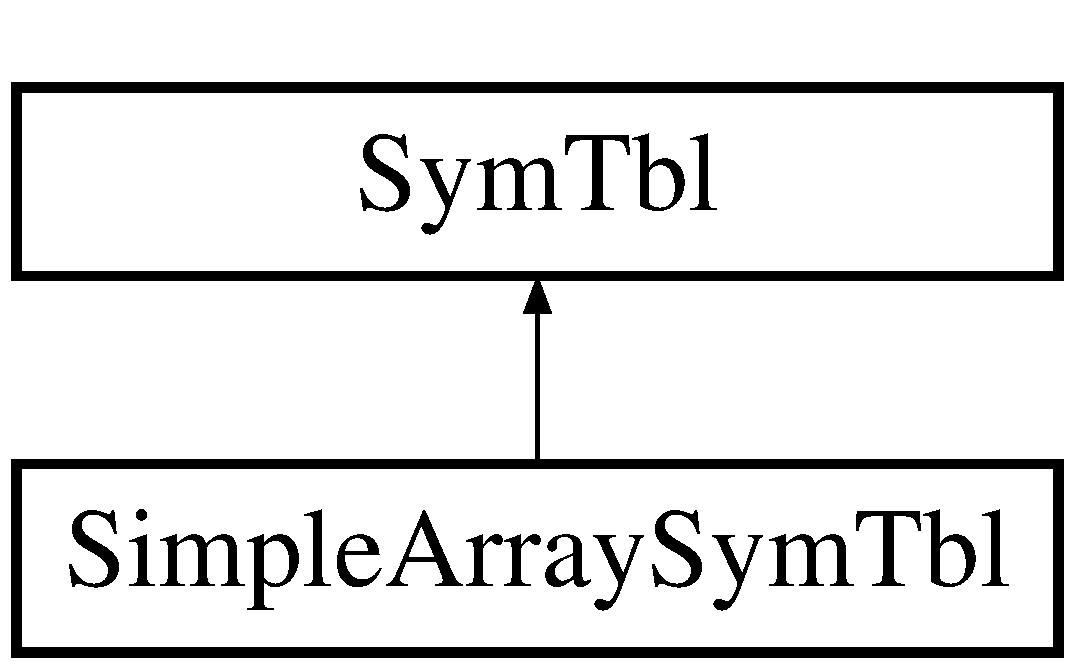
\includegraphics[height=2.000000cm]{class_sym_tbl}
\end{center}
\end{figure}
\subsection*{Public Member Functions}
\begin{DoxyCompactItemize}
\item 
virtual \hyperlink{class_var_address}{Var\+Address} $\ast$ \hyperlink{class_sym_tbl_a7cdd50cd38f3eecf23c9e6ce0c1696da}{get} (const char $\ast$lexeme)=0
\item 
virtual void \hyperlink{class_sym_tbl_a116640842b4776c1bacc6292b3015078}{put} (const char $\ast$lexeme, \hyperlink{tinycomp_8h_aca554671f4620139c1393f96d2af74bc}{type\+Name} type)=0
\item 
void \hyperlink{class_sym_tbl_a97e36880f52532dfac7367b2034e3346}{print\+Out} ()
\end{DoxyCompactItemize}
\subsection*{Protected Attributes}
\begin{DoxyCompactItemize}
\item 
\hyperlink{class_memory}{Memory} \& \hyperlink{class_sym_tbl_aacdfc3edb6f9bd947ea5bc7b5b695757}{mem} = \hyperlink{class_memory_a96eac3970b3baba973645a9cc32aee4c}{Memory\+::get\+Instance}()
\end{DoxyCompactItemize}
\subsection*{Friends}
\begin{DoxyCompactItemize}
\item 
void {\bfseries Memory\+::print\+Out} (\hyperlink{class_sym_tbl}{Sym\+Tbl} $\ast$tbl)\hypertarget{class_sym_tbl_ad9233821b14854177e4680a1ccad4f29}{}\label{class_sym_tbl_ad9233821b14854177e4680a1ccad4f29}

\end{DoxyCompactItemize}


\subsection{Detailed Description}
An abstraction for the Symbol Table 

\subsection{Member Function Documentation}
\index{Sym\+Tbl@{Sym\+Tbl}!get@{get}}
\index{get@{get}!Sym\+Tbl@{Sym\+Tbl}}
\subsubsection[{\texorpdfstring{get(const char $\ast$lexeme)=0}{get(const char *lexeme)=0}}]{\setlength{\rightskip}{0pt plus 5cm}virtual {\bf Var\+Address}$\ast$ Sym\+Tbl\+::get (
\begin{DoxyParamCaption}
\item[{const char $\ast$}]{lexeme}
\end{DoxyParamCaption}
)\hspace{0.3cm}{\ttfamily [pure virtual]}}\hypertarget{class_sym_tbl_a7cdd50cd38f3eecf23c9e6ce0c1696da}{}\label{class_sym_tbl_a7cdd50cd38f3eecf23c9e6ce0c1696da}
Pure virtual method; retrieves a variable from the symbol table. 
\begin{DoxyParams}{Parameters}
{\em lexeme} & The lexeme used as a key to access the symbol table \\
\hline
\end{DoxyParams}


Implemented in \hyperlink{class_simple_array_sym_tbl_a28d6d5c513f7b8f2beee3a0cf6eab45b}{Simple\+Array\+Sym\+Tbl}.

\index{Sym\+Tbl@{Sym\+Tbl}!print\+Out@{print\+Out}}
\index{print\+Out@{print\+Out}!Sym\+Tbl@{Sym\+Tbl}}
\subsubsection[{\texorpdfstring{print\+Out()}{printOut()}}]{\setlength{\rightskip}{0pt plus 5cm}void Sym\+Tbl\+::print\+Out (
\begin{DoxyParamCaption}
{}
\end{DoxyParamCaption}
)\hspace{0.3cm}{\ttfamily [inline]}}\hypertarget{class_sym_tbl_a97e36880f52532dfac7367b2034e3346}{}\label{class_sym_tbl_a97e36880f52532dfac7367b2034e3346}
Prints out the symbol table \index{Sym\+Tbl@{Sym\+Tbl}!put@{put}}
\index{put@{put}!Sym\+Tbl@{Sym\+Tbl}}
\subsubsection[{\texorpdfstring{put(const char $\ast$lexeme, type\+Name type)=0}{put(const char *lexeme, typeName type)=0}}]{\setlength{\rightskip}{0pt plus 5cm}virtual void Sym\+Tbl\+::put (
\begin{DoxyParamCaption}
\item[{const char $\ast$}]{lexeme, }
\item[{{\bf type\+Name}}]{type}
\end{DoxyParamCaption}
)\hspace{0.3cm}{\ttfamily [pure virtual]}}\hypertarget{class_sym_tbl_a116640842b4776c1bacc6292b3015078}{}\label{class_sym_tbl_a116640842b4776c1bacc6292b3015078}
Pure virtual method; stores a variable into the symbol table. 
\begin{DoxyParams}{Parameters}
{\em lexeme} & The lexeme used as a key to access the symbol table \\
\hline
{\em type} & The type of the lexeme \\
\hline
\end{DoxyParams}


Implemented in \hyperlink{class_simple_array_sym_tbl_ac7a485531efeaf7b6ac6b5215e212a37}{Simple\+Array\+Sym\+Tbl}.



\subsection{Field Documentation}
\index{Sym\+Tbl@{Sym\+Tbl}!mem@{mem}}
\index{mem@{mem}!Sym\+Tbl@{Sym\+Tbl}}
\subsubsection[{\texorpdfstring{mem}{mem}}]{\setlength{\rightskip}{0pt plus 5cm}{\bf Memory}\& Sym\+Tbl\+::mem = {\bf Memory\+::get\+Instance}()\hspace{0.3cm}{\ttfamily [protected]}}\hypertarget{class_sym_tbl_aacdfc3edb6f9bd947ea5bc7b5b695757}{}\label{class_sym_tbl_aacdfc3edb6f9bd947ea5bc7b5b695757}
A reference to the (simulated) memory 

The documentation for this class was generated from the following file\+:\begin{DoxyCompactItemize}
\item 
\hyperlink{tinycomp_8hpp}{tinycomp.\+hpp}\end{DoxyCompactItemize}

\hypertarget{class_tac_instr}{}\section{Tac\+Instr Class Reference}
\label{class_tac_instr}\index{Tac\+Instr@{Tac\+Instr}}


{\ttfamily \#include $<$tinycomp.\+hpp$>$}

\subsection*{Public Member Functions}
\begin{DoxyCompactItemize}
\item 
\hyperlink{class_tac_instr_ab607b7ce5c1f93748859e801eb6583a1}{Tac\+Instr} (\hyperlink{tinycomp_8h_a042125b56c7cb23c8c11e3aeb8de20cc}{opr\+Enum} op, \hyperlink{class_address}{Address} $\ast$operand1, \hyperlink{class_address}{Address} $\ast$operand2, \hyperlink{class_address}{Address} $\ast$operand3)
\item 
\hyperlink{tinycomp_8h_a042125b56c7cb23c8c11e3aeb8de20cc}{opr\+Enum} \hyperlink{class_tac_instr_afdf3f5b13808a3e8a73cfb8475f770e3}{get\+Op} () const 
\item 
\hyperlink{class_instr_address}{Instr\+Address} $\ast$ \hyperlink{class_tac_instr_ac4d3bc015e93338b0bba8af680576e30}{get\+Value\+Number} ()
\item 
void \hyperlink{class_tac_instr_a6e6955830a1420096bfc53be040675e9}{patch} (\hyperlink{class_tac_instr}{Tac\+Instr} $\ast$)
\end{DoxyCompactItemize}
\subsection*{Friends}
\begin{DoxyCompactItemize}
\item 
class {\bfseries Target\+Code}\hypertarget{class_tac_instr_a4a2d7047235cb01678f9f261600e3865}{}\label{class_tac_instr_a4a2d7047235cb01678f9f261600e3865}

\item 
std\+::ostream \& {\bfseries operator$<$$<$} (std\+::ostream \&, const \hyperlink{class_tac_instr}{Tac\+Instr} $\ast$)\hypertarget{class_tac_instr_a4497e4e38cff2ae7a1d600ee5e79bf87}{}\label{class_tac_instr_a4497e4e38cff2ae7a1d600ee5e79bf87}

\end{DoxyCompactItemize}


\subsection{Detailed Description}
A generic three-\/address code instruction. It will store\+:
\begin{DoxyItemize}
\item the instruction\textquotesingle{}s valuenumber
\item the operator \begin{DoxySeeAlso}{See also}
\hyperlink{tinycomp_8h_a042125b56c7cb23c8c11e3aeb8de20cc}{opr\+Enum} 
\end{DoxySeeAlso}

\end{DoxyItemize}

\subsection{Constructor \& Destructor Documentation}
\index{Tac\+Instr@{Tac\+Instr}!Tac\+Instr@{Tac\+Instr}}
\index{Tac\+Instr@{Tac\+Instr}!Tac\+Instr@{Tac\+Instr}}
\subsubsection[{\texorpdfstring{Tac\+Instr(opr\+Enum op, Address $\ast$operand1, Address $\ast$operand2, Address $\ast$operand3)}{TacInstr(oprEnum op, Address *operand1, Address *operand2, Address *operand3)}}]{\setlength{\rightskip}{0pt plus 5cm}Tac\+Instr\+::\+Tac\+Instr (
\begin{DoxyParamCaption}
\item[{{\bf opr\+Enum}}]{op, }
\item[{{\bf Address} $\ast$}]{operand1, }
\item[{{\bf Address} $\ast$}]{operand2, }
\item[{{\bf Address} $\ast$}]{operand3}
\end{DoxyParamCaption}
)}\hypertarget{class_tac_instr_ab607b7ce5c1f93748859e801eb6583a1}{}\label{class_tac_instr_ab607b7ce5c1f93748859e801eb6583a1}
Constructor of a 3-\/address code instruction. The result is internally stored as an \hyperlink{class_instr_address}{Instr\+Address} representing the value number (e.\+g corresponding to an index to the code array) 
\begin{DoxyParams}{Parameters}
{\em op} & The operator for this instruction, as an opr\+Enum \\
\hline
{\em operand1} & The first operand, as a generic \hyperlink{class_address}{Address} \\
\hline
{\em operand2} & The second operand (may be N\+U\+LL for operators that do not require 2 operands) \\
\hline
{\em operand3} & Holds a temporary, when explicitly needed to specify the address result, depending on the operation \\
\hline
\end{DoxyParams}


\subsection{Member Function Documentation}
\index{Tac\+Instr@{Tac\+Instr}!get\+Op@{get\+Op}}
\index{get\+Op@{get\+Op}!Tac\+Instr@{Tac\+Instr}}
\subsubsection[{\texorpdfstring{get\+Op() const }{getOp() const }}]{\setlength{\rightskip}{0pt plus 5cm}{\bf opr\+Enum} Tac\+Instr\+::get\+Op (
\begin{DoxyParamCaption}
{}
\end{DoxyParamCaption}
) const}\hypertarget{class_tac_instr_afdf3f5b13808a3e8a73cfb8475f770e3}{}\label{class_tac_instr_afdf3f5b13808a3e8a73cfb8475f770e3}
Returns the enum representing the operator of this specific instruction \index{Tac\+Instr@{Tac\+Instr}!get\+Value\+Number@{get\+Value\+Number}}
\index{get\+Value\+Number@{get\+Value\+Number}!Tac\+Instr@{Tac\+Instr}}
\subsubsection[{\texorpdfstring{get\+Value\+Number()}{getValueNumber()}}]{\setlength{\rightskip}{0pt plus 5cm}{\bf Instr\+Address}$\ast$ Tac\+Instr\+::get\+Value\+Number (
\begin{DoxyParamCaption}
{}
\end{DoxyParamCaption}
)}\hypertarget{class_tac_instr_ac4d3bc015e93338b0bba8af680576e30}{}\label{class_tac_instr_ac4d3bc015e93338b0bba8af680576e30}
Returns the \hyperlink{class_instr_address}{Instr\+Address} representing the value number \index{Tac\+Instr@{Tac\+Instr}!patch@{patch}}
\index{patch@{patch}!Tac\+Instr@{Tac\+Instr}}
\subsubsection[{\texorpdfstring{patch(\+Tac\+Instr $\ast$)}{patch(TacInstr *)}}]{\setlength{\rightskip}{0pt plus 5cm}void Tac\+Instr\+::patch (
\begin{DoxyParamCaption}
\item[{{\bf Tac\+Instr} $\ast$}]{}
\end{DoxyParamCaption}
)}\hypertarget{class_tac_instr_a6e6955830a1420096bfc53be040675e9}{}\label{class_tac_instr_a6e6955830a1420096bfc53be040675e9}
For backpathcing \char`\"{}goto\char`\"{}-\/like instructions 

The documentation for this class was generated from the following file\+:\begin{DoxyCompactItemize}
\item 
\hyperlink{tinycomp_8hpp}{tinycomp.\+hpp}\end{DoxyCompactItemize}

\hypertarget{class_target_code}{}\section{Target\+Code Class Reference}
\label{class_target_code}\index{Target\+Code@{Target\+Code}}


{\ttfamily \#include $<$tinycomp.\+hpp$>$}

\subsection*{Public Member Functions}
\begin{DoxyCompactItemize}
\item 
\hyperlink{class_target_code_ac5d1d427ace51cd109c586279543db80}{Target\+Code} ()
\item 
\hyperlink{class_tac_instr}{Tac\+Instr} $\ast$ \hyperlink{class_target_code_a4071467d8e74b5eaf495375cb3e4e2c0}{get\+Instr} (int i)
\item 
int \hyperlink{class_target_code_af38db8dcd404aab0757238b8634a2dbf}{get\+Next\+Instr} ()
\item 
\hyperlink{class_tac_instr}{Tac\+Instr} $\ast$ \hyperlink{class_target_code_a04e3ad62e9ead1c9237f1ba0d90e7b83}{gen} (\hyperlink{tinycomp_8h_a042125b56c7cb23c8c11e3aeb8de20cc}{opr\+Enum} op, \hyperlink{class_address}{Address} $\ast$operand1, \hyperlink{class_address}{Address} $\ast$operand2)
\item 
\hyperlink{class_tac_instr}{Tac\+Instr} $\ast$ \hyperlink{class_target_code_aff3458f28e2175256063869c4ee688f6}{gen} (\hyperlink{tinycomp_8h_a042125b56c7cb23c8c11e3aeb8de20cc}{opr\+Enum} op, \hyperlink{class_address}{Address} $\ast$operand1, \hyperlink{class_address}{Address} $\ast$operand2, \hyperlink{class_address}{Address} $\ast$operand3)
\item 
void \hyperlink{class_target_code_a8930a15f8287301265e46ba5dc5d6fe0}{backpatch} (list$<$ \hyperlink{class_tac_instr}{Tac\+Instr} $\ast$ $>$ gotolist, \hyperlink{class_tac_instr}{Tac\+Instr} $\ast$instr)
\item 
void \hyperlink{class_target_code_a252a90959cffeeff1c93cfb3e47c5ab9}{print\+Out} ()
\end{DoxyCompactItemize}


\subsection{Detailed Description}
A simplified abstraction for representing our target code. Following the textbook, I\textquotesingle{}m using 3-\/addr code instructions and storing them in an actual array. 

\subsection{Constructor \& Destructor Documentation}
\index{Target\+Code@{Target\+Code}!Target\+Code@{Target\+Code}}
\index{Target\+Code@{Target\+Code}!Target\+Code@{Target\+Code}}
\subsubsection[{\texorpdfstring{Target\+Code()}{TargetCode()}}]{\setlength{\rightskip}{0pt plus 5cm}Target\+Code\+::\+Target\+Code (
\begin{DoxyParamCaption}
{}
\end{DoxyParamCaption}
)}\hypertarget{class_target_code_ac5d1d427ace51cd109c586279543db80}{}\label{class_target_code_ac5d1d427ace51cd109c586279543db80}
Basic constructor; it will initialize the internal array of \hyperlink{class_tac_instr}{Tac\+Instr} instructions 

\subsection{Member Function Documentation}
\index{Target\+Code@{Target\+Code}!backpatch@{backpatch}}
\index{backpatch@{backpatch}!Target\+Code@{Target\+Code}}
\subsubsection[{\texorpdfstring{backpatch(list$<$ Tac\+Instr $\ast$ $>$ gotolist, Tac\+Instr $\ast$instr)}{backpatch(list< TacInstr * > gotolist, TacInstr *instr)}}]{\setlength{\rightskip}{0pt plus 5cm}void Target\+Code\+::backpatch (
\begin{DoxyParamCaption}
\item[{list$<$ {\bf Tac\+Instr} $\ast$ $>$}]{gotolist, }
\item[{{\bf Tac\+Instr} $\ast$}]{instr}
\end{DoxyParamCaption}
)}\hypertarget{class_target_code_a8930a15f8287301265e46ba5dc5d6fe0}{}\label{class_target_code_a8930a15f8287301265e46ba5dc5d6fe0}
Implementation of \char`\"{}backpatch()\char`\"{} from the textbook. 
\begin{DoxyParams}{Parameters}
{\em gotolist} & a list of \hyperlink{class_tac_instr}{Tac\+Instr}; each one is assumed to be a \char`\"{}goto\char`\"{}-\/like instruction \\
\hline
{\em instr} & the \hyperlink{class_address}{Address} of the instruction (i.\+e. \hyperlink{class_tac_instr}{Tac\+Instr}) to be patched in the goto\textquotesingle{}s in the list \\
\hline
\end{DoxyParams}
\index{Target\+Code@{Target\+Code}!gen@{gen}}
\index{gen@{gen}!Target\+Code@{Target\+Code}}
\subsubsection[{\texorpdfstring{gen(opr\+Enum op, Address $\ast$operand1, Address $\ast$operand2)}{gen(oprEnum op, Address *operand1, Address *operand2)}}]{\setlength{\rightskip}{0pt plus 5cm}{\bf Tac\+Instr}$\ast$ Target\+Code\+::gen (
\begin{DoxyParamCaption}
\item[{{\bf opr\+Enum}}]{op, }
\item[{{\bf Address} $\ast$}]{operand1, }
\item[{{\bf Address} $\ast$}]{operand2}
\end{DoxyParamCaption}
)}\hypertarget{class_target_code_a04e3ad62e9ead1c9237f1ba0d90e7b83}{}\label{class_target_code_a04e3ad62e9ead1c9237f1ba0d90e7b83}
Implementation of \char`\"{}gen()\char`\"{} from the textbook. Basically, if generates a new \hyperlink{class_tac_instr}{Tac\+Instr} with the given parameters, and stores it in the next available place in the code array \index{Target\+Code@{Target\+Code}!gen@{gen}}
\index{gen@{gen}!Target\+Code@{Target\+Code}}
\subsubsection[{\texorpdfstring{gen(opr\+Enum op, Address $\ast$operand1, Address $\ast$operand2, Address $\ast$operand3)}{gen(oprEnum op, Address *operand1, Address *operand2, Address *operand3)}}]{\setlength{\rightskip}{0pt plus 5cm}{\bf Tac\+Instr}$\ast$ Target\+Code\+::gen (
\begin{DoxyParamCaption}
\item[{{\bf opr\+Enum}}]{op, }
\item[{{\bf Address} $\ast$}]{operand1, }
\item[{{\bf Address} $\ast$}]{operand2, }
\item[{{\bf Address} $\ast$}]{operand3}
\end{DoxyParamCaption}
)}\hypertarget{class_target_code_aff3458f28e2175256063869c4ee688f6}{}\label{class_target_code_aff3458f28e2175256063869c4ee688f6}
Implementation of \char`\"{}gen()\char`\"{} from the textbook. Basically, if generates a new \hyperlink{class_tac_instr}{Tac\+Instr} with the given parameters, and stores it in the next available place in the code array This version accounts for using temporaries. \index{Target\+Code@{Target\+Code}!get\+Instr@{get\+Instr}}
\index{get\+Instr@{get\+Instr}!Target\+Code@{Target\+Code}}
\subsubsection[{\texorpdfstring{get\+Instr(int i)}{getInstr(int i)}}]{\setlength{\rightskip}{0pt plus 5cm}{\bf Tac\+Instr}$\ast$ Target\+Code\+::get\+Instr (
\begin{DoxyParamCaption}
\item[{int}]{i}
\end{DoxyParamCaption}
)}\hypertarget{class_target_code_a4071467d8e74b5eaf495375cb3e4e2c0}{}\label{class_target_code_a4071467d8e74b5eaf495375cb3e4e2c0}
Returns the instruction stored at index i in the code array \index{Target\+Code@{Target\+Code}!get\+Next\+Instr@{get\+Next\+Instr}}
\index{get\+Next\+Instr@{get\+Next\+Instr}!Target\+Code@{Target\+Code}}
\subsubsection[{\texorpdfstring{get\+Next\+Instr()}{getNextInstr()}}]{\setlength{\rightskip}{0pt plus 5cm}int Target\+Code\+::get\+Next\+Instr (
\begin{DoxyParamCaption}
{}
\end{DoxyParamCaption}
)}\hypertarget{class_target_code_af38db8dcd404aab0757238b8634a2dbf}{}\label{class_target_code_af38db8dcd404aab0757238b8634a2dbf}
Implementation of \char`\"{}nextinstr\char`\"{} from the textbook \index{Target\+Code@{Target\+Code}!print\+Out@{print\+Out}}
\index{print\+Out@{print\+Out}!Target\+Code@{Target\+Code}}
\subsubsection[{\texorpdfstring{print\+Out()}{printOut()}}]{\setlength{\rightskip}{0pt plus 5cm}void Target\+Code\+::print\+Out (
\begin{DoxyParamCaption}
{}
\end{DoxyParamCaption}
)}\hypertarget{class_target_code_a252a90959cffeeff1c93cfb3e47c5ab9}{}\label{class_target_code_a252a90959cffeeff1c93cfb3e47c5ab9}
A convenience method to print out the entire code array 

The documentation for this class was generated from the following file\+:\begin{DoxyCompactItemize}
\item 
\hyperlink{tinycomp_8hpp}{tinycomp.\+hpp}\end{DoxyCompactItemize}

\hypertarget{class_temp_address}{}\section{Temp\+Address Class Reference}
\label{class_temp_address}\index{Temp\+Address@{Temp\+Address}}


{\ttfamily \#include $<$tinycomp.\+hpp$>$}

Inheritance diagram for Temp\+Address\+:\begin{figure}[H]
\begin{center}
\leavevmode
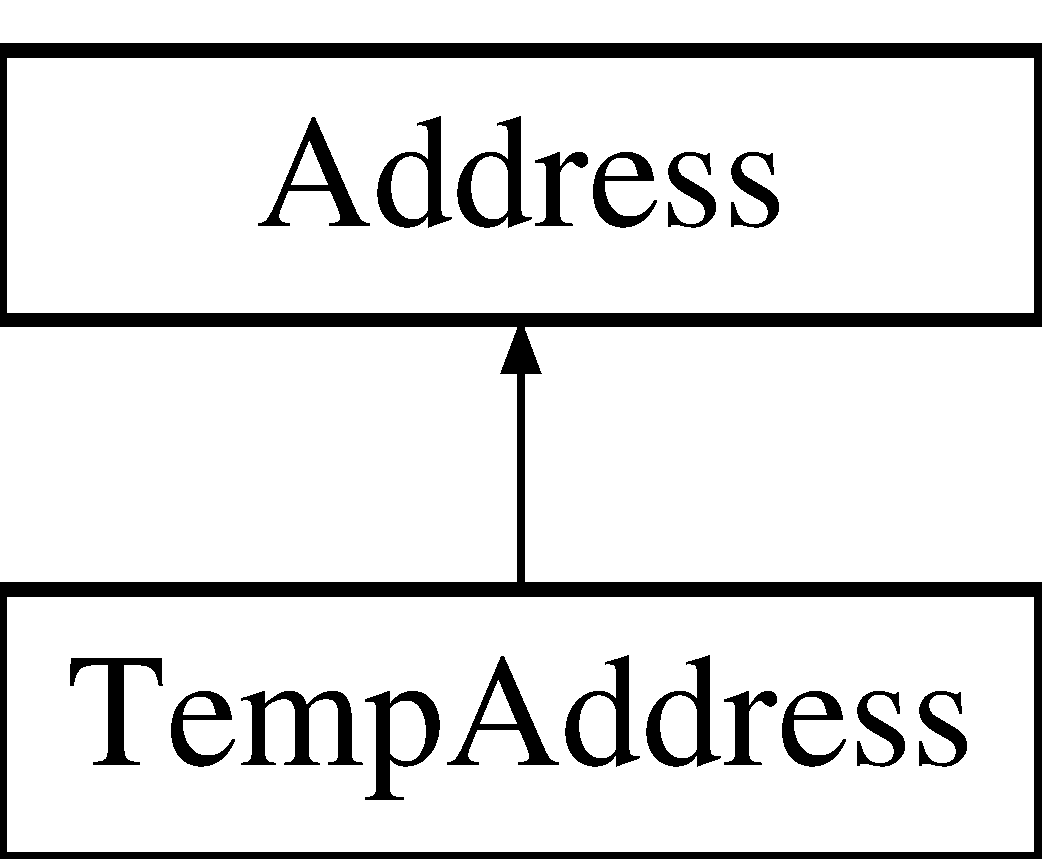
\includegraphics[height=2.000000cm]{class_temp_address}
\end{center}
\end{figure}
\subsection*{Public Member Functions}
\begin{DoxyCompactItemize}
\item 
int \hyperlink{class_temp_address_ac6b8829b9c189545a43a05fdc9da6206}{get\+Offset} ()
\item 
const char $\ast$ \hyperlink{class_temp_address_a553ea130e6d932490fedc2da9cdb87b6}{to\+String} () const 
\end{DoxyCompactItemize}
\subsection*{Additional Inherited Members}


\subsection{Detailed Description}
A specialization of \hyperlink{class_address}{Address} to hold a temporary 

\subsection{Member Function Documentation}
\index{Temp\+Address@{Temp\+Address}!get\+Offset@{get\+Offset}}
\index{get\+Offset@{get\+Offset}!Temp\+Address@{Temp\+Address}}
\subsubsection[{\texorpdfstring{get\+Offset()}{getOffset()}}]{\setlength{\rightskip}{0pt plus 5cm}int Temp\+Address\+::get\+Offset (
\begin{DoxyParamCaption}
{}
\end{DoxyParamCaption}
)}\hypertarget{class_temp_address_ac6b8829b9c189545a43a05fdc9da6206}{}\label{class_temp_address_ac6b8829b9c189545a43a05fdc9da6206}
Returns the pointer to the memory location holding the temporary \index{Temp\+Address@{Temp\+Address}!to\+String@{to\+String}}
\index{to\+String@{to\+String}!Temp\+Address@{Temp\+Address}}
\subsubsection[{\texorpdfstring{to\+String() const }{toString() const }}]{\setlength{\rightskip}{0pt plus 5cm}const char$\ast$ Temp\+Address\+::to\+String (
\begin{DoxyParamCaption}
{}
\end{DoxyParamCaption}
) const\hspace{0.3cm}{\ttfamily [virtual]}}\hypertarget{class_temp_address_a553ea130e6d932490fedc2da9cdb87b6}{}\label{class_temp_address_a553ea130e6d932490fedc2da9cdb87b6}
Concrete method for printing a \hyperlink{class_temp_address}{Temp\+Address}; it\textquotesingle{}s a concrete implementation of the corresponding abstract method in \hyperlink{class_address}{Address} 

Implements \hyperlink{class_address_ac58183c3d3dc7c3e98a17825dd086de1}{Address}.



The documentation for this class was generated from the following file\+:\begin{DoxyCompactItemize}
\item 
\hyperlink{tinycomp_8hpp}{tinycomp.\+hpp}\end{DoxyCompactItemize}

\hypertarget{class_var_address}{}\section{Var\+Address Class Reference}
\label{class_var_address}\index{Var\+Address@{Var\+Address}}


{\ttfamily \#include $<$tinycomp.\+hpp$>$}

Inheritance diagram for Var\+Address\+:\begin{figure}[H]
\begin{center}
\leavevmode
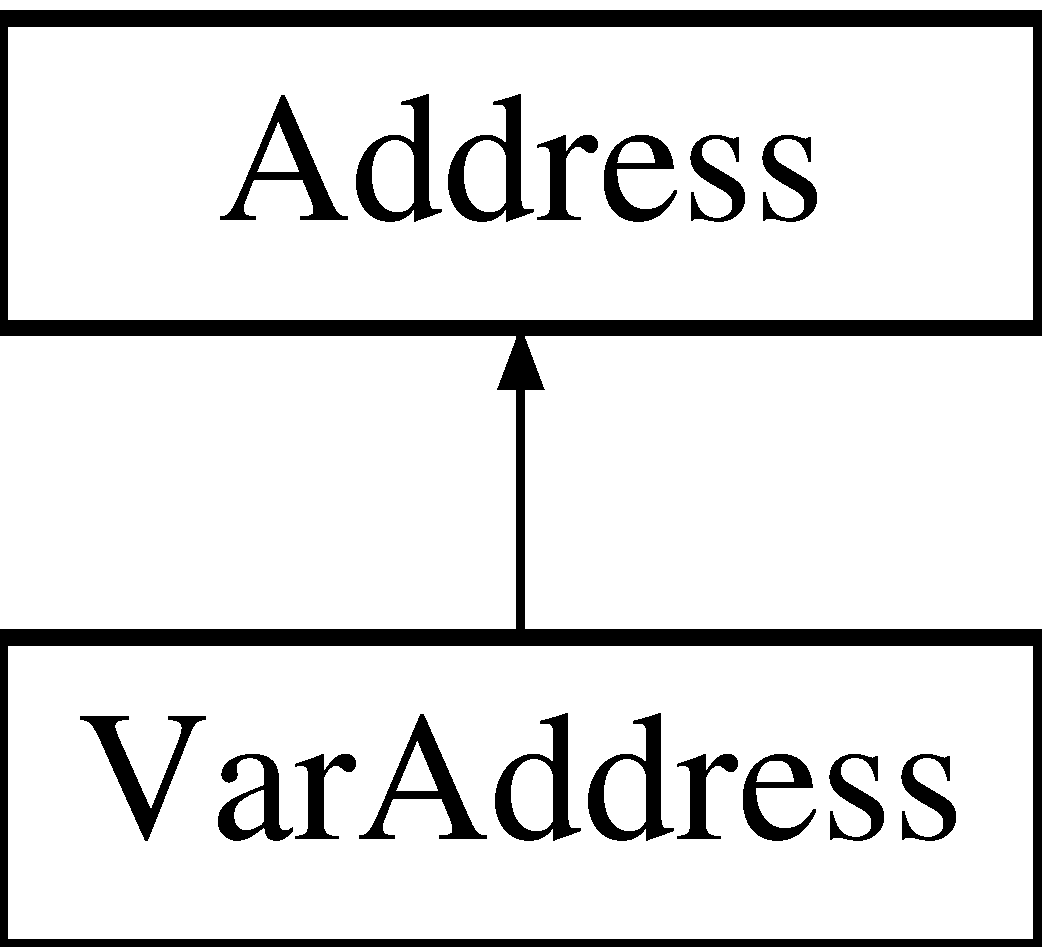
\includegraphics[height=2.000000cm]{class_var_address}
\end{center}
\end{figure}
\subsection*{Public Member Functions}
\begin{DoxyCompactItemize}
\item 
\hyperlink{class_var_address_ac99b3b4bc40e6dc1a4f0dede68d858cf}{Var\+Address} (char v, \hyperlink{tinycomp_8h_aca554671f4620139c1393f96d2af74bc}{type\+Name} t, int offset)
\item 
\hyperlink{tinycomp_8h_aca554671f4620139c1393f96d2af74bc}{type\+Name} \hyperlink{class_var_address_a01ec05b9f9e33978980d6ad676154a91}{get\+Type} ()
\item 
int \hyperlink{class_var_address_aa3b8cd6699634ac705fc2dea982e0b87}{get\+Width} ()
\item 
int \hyperlink{class_var_address_a825ed81c1a17b3d374999f0457a35a48}{get\+Offset} ()
\item 
const char $\ast$ \hyperlink{class_var_address_abadfe890b239f9dcc5ae5bbe31626d49}{to\+String} () const 
\end{DoxyCompactItemize}
\subsection*{Additional Inherited Members}


\subsection{Detailed Description}
A specialization of \hyperlink{class_address}{Address} to hold a variable 

\subsection{Constructor \& Destructor Documentation}
\index{Var\+Address@{Var\+Address}!Var\+Address@{Var\+Address}}
\index{Var\+Address@{Var\+Address}!Var\+Address@{Var\+Address}}
\subsubsection[{\texorpdfstring{Var\+Address(char v, type\+Name t, int offset)}{VarAddress(char v, typeName t, int offset)}}]{\setlength{\rightskip}{0pt plus 5cm}Var\+Address\+::\+Var\+Address (
\begin{DoxyParamCaption}
\item[{char}]{v, }
\item[{{\bf type\+Name}}]{t, }
\item[{int}]{offset}
\end{DoxyParamCaption}
)}\hypertarget{class_var_address_ac99b3b4bc40e6dc1a4f0dede68d858cf}{}\label{class_var_address_ac99b3b4bc40e6dc1a4f0dede68d858cf}
Constructor\+: creates a variable address from its id (assuming only 1-\/char id\textquotesingle{}s). 

\subsection{Member Function Documentation}
\index{Var\+Address@{Var\+Address}!get\+Offset@{get\+Offset}}
\index{get\+Offset@{get\+Offset}!Var\+Address@{Var\+Address}}
\subsubsection[{\texorpdfstring{get\+Offset()}{getOffset()}}]{\setlength{\rightskip}{0pt plus 5cm}int Var\+Address\+::get\+Offset (
\begin{DoxyParamCaption}
{}
\end{DoxyParamCaption}
)}\hypertarget{class_var_address_a825ed81c1a17b3d374999f0457a35a48}{}\label{class_var_address_a825ed81c1a17b3d374999f0457a35a48}
Returns the pointer to the memory location holding the variable\textquotesingle{}s value \index{Var\+Address@{Var\+Address}!get\+Type@{get\+Type}}
\index{get\+Type@{get\+Type}!Var\+Address@{Var\+Address}}
\subsubsection[{\texorpdfstring{get\+Type()}{getType()}}]{\setlength{\rightskip}{0pt plus 5cm}{\bf type\+Name} Var\+Address\+::get\+Type (
\begin{DoxyParamCaption}
{}
\end{DoxyParamCaption}
)}\hypertarget{class_var_address_a01ec05b9f9e33978980d6ad676154a91}{}\label{class_var_address_a01ec05b9f9e33978980d6ad676154a91}
Returns the variable\textquotesingle{}s type (as a type\+Name enum) \index{Var\+Address@{Var\+Address}!get\+Width@{get\+Width}}
\index{get\+Width@{get\+Width}!Var\+Address@{Var\+Address}}
\subsubsection[{\texorpdfstring{get\+Width()}{getWidth()}}]{\setlength{\rightskip}{0pt plus 5cm}int Var\+Address\+::get\+Width (
\begin{DoxyParamCaption}
{}
\end{DoxyParamCaption}
)}\hypertarget{class_var_address_aa3b8cd6699634ac705fc2dea982e0b87}{}\label{class_var_address_aa3b8cd6699634ac705fc2dea982e0b87}
Returns the variable\textquotesingle{}s width, which depends on its type \index{Var\+Address@{Var\+Address}!to\+String@{to\+String}}
\index{to\+String@{to\+String}!Var\+Address@{Var\+Address}}
\subsubsection[{\texorpdfstring{to\+String() const }{toString() const }}]{\setlength{\rightskip}{0pt plus 5cm}const char$\ast$ Var\+Address\+::to\+String (
\begin{DoxyParamCaption}
{}
\end{DoxyParamCaption}
) const\hspace{0.3cm}{\ttfamily [virtual]}}\hypertarget{class_var_address_abadfe890b239f9dcc5ae5bbe31626d49}{}\label{class_var_address_abadfe890b239f9dcc5ae5bbe31626d49}
Concrete method for printing a \hyperlink{class_var_address}{Var\+Address}; it\textquotesingle{}s a concrete implementation of the corresponding abstract method in \hyperlink{class_address}{Address} 

Implements \hyperlink{class_address_ac58183c3d3dc7c3e98a17825dd086de1}{Address}.



The documentation for this class was generated from the following file\+:\begin{DoxyCompactItemize}
\item 
\hyperlink{tinycomp_8hpp}{tinycomp.\+hpp}\end{DoxyCompactItemize}

\chapter{File Documentation}
\hypertarget{tinycomp_8h}{}\section{tinycomp.\+h File Reference}
\label{tinycomp_8h}\index{tinycomp.\+h@{tinycomp.\+h}}


This header file contains the definitions that must be shared between flex, bison, and the support code.  


\subsection*{Data Structures}
\begin{DoxyCompactItemize}
\item 
struct \hyperlink{structfraction}{fraction}
\item 
class \hyperlink{class_attribute}{Attribute}
\end{DoxyCompactItemize}
\subsection*{Enumerations}
\begin{DoxyCompactItemize}
\item 
enum \hyperlink{tinycomp_8h_aca554671f4620139c1393f96d2af74bc}{type\+Name} \{ \hyperlink{tinycomp_8h_aca554671f4620139c1393f96d2af74bca9141d27e9f536d86b3fe96734107bb1f}{int\+Type}, 
\hyperlink{tinycomp_8h_aca554671f4620139c1393f96d2af74bcaf3dc8496c1283a092729d6ce1073bc8a}{float\+Type}, 
{\bfseries fraction\+Type}
 \}
\item 
enum \hyperlink{tinycomp_8h_a042125b56c7cb23c8c11e3aeb8de20cc}{opr\+Enum} \{ \\*
\hyperlink{tinycomp_8h_a042125b56c7cb23c8c11e3aeb8de20ccae9609c8f75169fb851505584b51d0702}{U\+N\+K\+N\+O\+W\+N\+Opr}, 
\hyperlink{tinycomp_8h_a042125b56c7cb23c8c11e3aeb8de20cca9ca42e1cdb09d5b9aebd48645a38ac2b}{halt\+Opr}, 
\hyperlink{tinycomp_8h_a042125b56c7cb23c8c11e3aeb8de20cca08e29344d1e6daec5dc74d67d75f7992}{copy\+Opr}, 
\hyperlink{tinycomp_8h_a042125b56c7cb23c8c11e3aeb8de20ccacd7e2d55db7d186b0d37814e57f79c88}{add\+Opr}, 
\\*
{\bfseries mul\+Opr}, 
\hyperlink{tinycomp_8h_a042125b56c7cb23c8c11e3aeb8de20cca7a4cd7ce369eeccc7271b950c984b528}{div\+Opr}, 
\hyperlink{tinycomp_8h_a042125b56c7cb23c8c11e3aeb8de20cca1ea2304a08a16a33700e86c4f13a69b7}{index\+Copy\+Opr}, 
\hyperlink{tinycomp_8h_a042125b56c7cb23c8c11e3aeb8de20cca994150a4971bf26010336b2cdc73d0a6}{offset\+Opr}, 
\\*
\hyperlink{tinycomp_8h_a042125b56c7cb23c8c11e3aeb8de20cca76f47ddb50665a12d1dc67a1093e993c}{jmp\+Opr}, 
\hyperlink{tinycomp_8h_a042125b56c7cb23c8c11e3aeb8de20ccad445b0051ac3cd13fba3a3aed1b796e6}{eq1cond\+Jmp\+Opr}, 
\hyperlink{tinycomp_8h_a042125b56c7cb23c8c11e3aeb8de20cca339df0491c20ede3dd0e43ddb9786e64}{eq2cond\+Jmp\+Opr}, 
\hyperlink{tinycomp_8h_a042125b56c7cb23c8c11e3aeb8de20ccadf70a4cfb045cb8486cec6bde50affb4}{fake\+Opr}
 \}
\end{DoxyCompactItemize}


\subsection{Detailed Description}
This header file contains the definitions that must be shared between flex, bison, and the support code. 

\begin{DoxyAuthor}{Author}
Marco Ortolani 
\end{DoxyAuthor}
\begin{DoxyDate}{Date}
3/13/2017 
\end{DoxyDate}


\subsection{Enumeration Type Documentation}
\index{tinycomp.\+h@{tinycomp.\+h}!opr\+Enum@{opr\+Enum}}
\index{opr\+Enum@{opr\+Enum}!tinycomp.\+h@{tinycomp.\+h}}
\subsubsection[{\texorpdfstring{opr\+Enum}{oprEnum}}]{\setlength{\rightskip}{0pt plus 5cm}enum {\bf opr\+Enum}}\hypertarget{tinycomp_8h_a042125b56c7cb23c8c11e3aeb8de20cc}{}\label{tinycomp_8h_a042125b56c7cb23c8c11e3aeb8de20cc}
Enums for 3-\/addr code -\/ operators \begin{Desc}
\item[Enumerator]\par
\begin{description}
\index{U\+N\+K\+N\+O\+W\+N\+Opr@{U\+N\+K\+N\+O\+W\+N\+Opr}!tinycomp.\+h@{tinycomp.\+h}}\index{tinycomp.\+h@{tinycomp.\+h}!U\+N\+K\+N\+O\+W\+N\+Opr@{U\+N\+K\+N\+O\+W\+N\+Opr}}\item[{\em 
U\+N\+K\+N\+O\+W\+N\+Opr\hypertarget{tinycomp_8h_a042125b56c7cb23c8c11e3aeb8de20ccae9609c8f75169fb851505584b51d0702}{}\label{tinycomp_8h_a042125b56c7cb23c8c11e3aeb8de20ccae9609c8f75169fb851505584b51d0702}
}]this is the default, for an unknown operator (it should not occur) \index{halt\+Opr@{halt\+Opr}!tinycomp.\+h@{tinycomp.\+h}}\index{tinycomp.\+h@{tinycomp.\+h}!halt\+Opr@{halt\+Opr}}\item[{\em 
halt\+Opr\hypertarget{tinycomp_8h_a042125b56c7cb23c8c11e3aeb8de20cca9ca42e1cdb09d5b9aebd48645a38ac2b}{}\label{tinycomp_8h_a042125b56c7cb23c8c11e3aeb8de20cca9ca42e1cdb09d5b9aebd48645a38ac2b}
}]return control to the operating system \index{copy\+Opr@{copy\+Opr}!tinycomp.\+h@{tinycomp.\+h}}\index{tinycomp.\+h@{tinycomp.\+h}!copy\+Opr@{copy\+Opr}}\item[{\em 
copy\+Opr\hypertarget{tinycomp_8h_a042125b56c7cb23c8c11e3aeb8de20cca08e29344d1e6daec5dc74d67d75f7992}{}\label{tinycomp_8h_a042125b56c7cb23c8c11e3aeb8de20cca08e29344d1e6daec5dc74d67d75f7992}
}]the assignment operator \index{add\+Opr@{add\+Opr}!tinycomp.\+h@{tinycomp.\+h}}\index{tinycomp.\+h@{tinycomp.\+h}!add\+Opr@{add\+Opr}}\item[{\em 
add\+Opr\hypertarget{tinycomp_8h_a042125b56c7cb23c8c11e3aeb8de20ccacd7e2d55db7d186b0d37814e57f79c88}{}\label{tinycomp_8h_a042125b56c7cb23c8c11e3aeb8de20ccacd7e2d55db7d186b0d37814e57f79c88}
}]the addition operator \index{div\+Opr@{div\+Opr}!tinycomp.\+h@{tinycomp.\+h}}\index{tinycomp.\+h@{tinycomp.\+h}!div\+Opr@{div\+Opr}}\item[{\em 
div\+Opr\hypertarget{tinycomp_8h_a042125b56c7cb23c8c11e3aeb8de20cca7a4cd7ce369eeccc7271b950c984b528}{}\label{tinycomp_8h_a042125b56c7cb23c8c11e3aeb8de20cca7a4cd7ce369eeccc7271b950c984b528}
}]the multiplication operator \index{index\+Copy\+Opr@{index\+Copy\+Opr}!tinycomp.\+h@{tinycomp.\+h}}\index{tinycomp.\+h@{tinycomp.\+h}!index\+Copy\+Opr@{index\+Copy\+Opr}}\item[{\em 
index\+Copy\+Opr\hypertarget{tinycomp_8h_a042125b56c7cb23c8c11e3aeb8de20cca1ea2304a08a16a33700e86c4f13a69b7}{}\label{tinycomp_8h_a042125b56c7cb23c8c11e3aeb8de20cca1ea2304a08a16a33700e86c4f13a69b7}
}]the indexed copy operator x\mbox{[}i\mbox{]} = y \index{offset\+Opr@{offset\+Opr}!tinycomp.\+h@{tinycomp.\+h}}\index{tinycomp.\+h@{tinycomp.\+h}!offset\+Opr@{offset\+Opr}}\item[{\em 
offset\+Opr\hypertarget{tinycomp_8h_a042125b56c7cb23c8c11e3aeb8de20cca994150a4971bf26010336b2cdc73d0a6}{}\label{tinycomp_8h_a042125b56c7cb23c8c11e3aeb8de20cca994150a4971bf26010336b2cdc73d0a6}
}]the displacement operator x = y\mbox{[}i\mbox{]} \index{jmp\+Opr@{jmp\+Opr}!tinycomp.\+h@{tinycomp.\+h}}\index{tinycomp.\+h@{tinycomp.\+h}!jmp\+Opr@{jmp\+Opr}}\item[{\em 
jmp\+Opr\hypertarget{tinycomp_8h_a042125b56c7cb23c8c11e3aeb8de20cca76f47ddb50665a12d1dc67a1093e993c}{}\label{tinycomp_8h_a042125b56c7cb23c8c11e3aeb8de20cca76f47ddb50665a12d1dc67a1093e993c}
}]unconditional jump; the goto operator \index{eq1cond\+Jmp\+Opr@{eq1cond\+Jmp\+Opr}!tinycomp.\+h@{tinycomp.\+h}}\index{tinycomp.\+h@{tinycomp.\+h}!eq1cond\+Jmp\+Opr@{eq1cond\+Jmp\+Opr}}\item[{\em 
eq1cond\+Jmp\+Opr\hypertarget{tinycomp_8h_a042125b56c7cb23c8c11e3aeb8de20ccad445b0051ac3cd13fba3a3aed1b796e6}{}\label{tinycomp_8h_a042125b56c7cb23c8c11e3aeb8de20ccad445b0051ac3cd13fba3a3aed1b796e6}
}]== operator \index{eq2cond\+Jmp\+Opr@{eq2cond\+Jmp\+Opr}!tinycomp.\+h@{tinycomp.\+h}}\index{tinycomp.\+h@{tinycomp.\+h}!eq2cond\+Jmp\+Opr@{eq2cond\+Jmp\+Opr}}\item[{\em 
eq2cond\+Jmp\+Opr\hypertarget{tinycomp_8h_a042125b56c7cb23c8c11e3aeb8de20cca339df0491c20ede3dd0e43ddb9786e64}{}\label{tinycomp_8h_a042125b56c7cb23c8c11e3aeb8de20cca339df0491c20ede3dd0e43ddb9786e64}
}]= operator \index{fake\+Opr@{fake\+Opr}!tinycomp.\+h@{tinycomp.\+h}}\index{tinycomp.\+h@{tinycomp.\+h}!fake\+Opr@{fake\+Opr}}\item[{\em 
fake\+Opr\hypertarget{tinycomp_8h_a042125b56c7cb23c8c11e3aeb8de20ccadf70a4cfb045cb8486cec6bde50affb4}{}\label{tinycomp_8h_a042125b56c7cb23c8c11e3aeb8de20ccadf70a4cfb045cb8486cec6bde50affb4}
}]a temporary \char`\"{}fake\char`\"{} operator for simulating the ones yet-\/to-\/be implemented \end{description}
\end{Desc}
\index{tinycomp.\+h@{tinycomp.\+h}!type\+Name@{type\+Name}}
\index{type\+Name@{type\+Name}!tinycomp.\+h@{tinycomp.\+h}}
\subsubsection[{\texorpdfstring{type\+Name}{typeName}}]{\setlength{\rightskip}{0pt plus 5cm}enum {\bf type\+Name}}\hypertarget{tinycomp_8h_aca554671f4620139c1393f96d2af74bc}{}\label{tinycomp_8h_aca554671f4620139c1393f96d2af74bc}
Type system; each native data type is stored as a value in this enumeration. Note that for structured types we need a more complex structure; also, I am not explicitly accounting for a type hierarchy here. \begin{Desc}
\item[Enumerator]\par
\begin{description}
\index{int\+Type@{int\+Type}!tinycomp.\+h@{tinycomp.\+h}}\index{tinycomp.\+h@{tinycomp.\+h}!int\+Type@{int\+Type}}\item[{\em 
int\+Type\hypertarget{tinycomp_8h_aca554671f4620139c1393f96d2af74bca9141d27e9f536d86b3fe96734107bb1f}{}\label{tinycomp_8h_aca554671f4620139c1393f96d2af74bca9141d27e9f536d86b3fe96734107bb1f}
}]integer type \index{float\+Type@{float\+Type}!tinycomp.\+h@{tinycomp.\+h}}\index{tinycomp.\+h@{tinycomp.\+h}!float\+Type@{float\+Type}}\item[{\em 
float\+Type\hypertarget{tinycomp_8h_aca554671f4620139c1393f96d2af74bcaf3dc8496c1283a092729d6ce1073bc8a}{}\label{tinycomp_8h_aca554671f4620139c1393f96d2af74bcaf3dc8496c1283a092729d6ce1073bc8a}
}]floating point type \end{description}
\end{Desc}

\hypertarget{tinycomp_8hpp}{}\section{tinycomp.\+hpp File Reference}
\label{tinycomp_8hpp}\index{tinycomp.\+hpp@{tinycomp.\+hpp}}


This header file contains the support code for the translator of tinycomp.  


{\ttfamily \#include $<$iostream$>$}\\*
{\ttfamily \#include $<$list$>$}\\*
{\ttfamily \#include \char`\"{}tinycomp.\+h\char`\"{}}\\*
\subsection*{Data Structures}
\begin{DoxyCompactItemize}
\item 
class \hyperlink{class_address}{Address}
\item 
class \hyperlink{class_const_address}{Const\+Address}
\item 
class \hyperlink{class_var_address}{Var\+Address}
\item 
class \hyperlink{class_temp_address}{Temp\+Address}
\item 
class \hyperlink{class_instr_address}{Instr\+Address}
\item 
class \hyperlink{class_tac_instr}{Tac\+Instr}
\item 
class \hyperlink{class_memory}{Memory}
\item 
class \hyperlink{class_target_code}{Target\+Code}
\item 
class \hyperlink{class_sym_tbl}{Sym\+Tbl}
\item 
class \hyperlink{class_simple_array_sym_tbl}{Simple\+Array\+Sym\+Tbl}
\item 
class \hyperlink{class_expr_attr}{Expr\+Attr}
\item 
class \hyperlink{class_bool_attr}{Bool\+Attr}
\item 
class \hyperlink{class_stmt_attr}{Stmt\+Attr}
\end{DoxyCompactItemize}


\subsection{Detailed Description}
This header file contains the support code for the translator of tinycomp. 

\begin{DoxyAuthor}{Author}
Marco Ortolani 
\end{DoxyAuthor}
\begin{DoxyDate}{Date}
3/13/2017 
\end{DoxyDate}

%--- End generated contents ---

% Index
\backmatter
\newpage
\phantomsection
\clearemptydoublepage
\addcontentsline{toc}{chapter}{Index}
\printindex

\end{document}
